\documentclass{beamer} % "Beamer" is a word used in Germany to mean video projector. 

\usetheme{Goettingen} % Search online for beamer themes to find your favorite or use the Berkeley theme as in this file.
\usecolortheme{lily}
				\usepackage{color} % It may be necessary to set PCTeX or whatever program you are using to output a .pdf instead of a .dvi file in order to see color on your screen.
\usepackage{graphicx} % This package is needed if you wish to include external image files.
\theoremstyle{definition} % See Lesson Three of the LaTeX Manual for more on this kind of "proclamation."
\setbeamertemplate{footline}[frame number]
%\usebeamerfont{institute in head/foot}\insertshortinstitute
\newtheorem*{dfn}{A Reasonable Definition}               
\title{EBA : Electricity Board Application}

\institute{College of Engineering, Cherthala}


\AtBeginSection[]  % The commands within the following {} will be executed at the start of each section.
{
\begin{frame} % Within each "frame" there will be one or more "slides."  
\frametitle{Presentation Outline} % This is the title of the outline.
\tableofcontents[currentsection]  % This will display the table of contents and highlight the current section.
\end{frame}
} % Do not include the preceding set of commands if you prefer not to have a recurring outline displayed during your presentation.





\begin{document}

%\begin{frame} 
\titlepage
%\item \centering Guide:Sreelekshmi Murali
%\item \centering Reg No:12143649
%\end{frame}




%\section{What Can Happen at a Critical Point?} % Since this is the start of a new section, our recurring outline will appear here.

\begin{frame}
\frametitle{GROUP 7}
\textbf{AJESH M (04)\\ MUHAMMED NADIRSHA N K (24)\\ RIBIN ROY (28)\\ SREENIVAS S NAIK(34)}
\begin{flushright}
\textbf{Guide: Mrs. Anitha M A }
\end{flushright}
\end{frame}
\begin{frame} 
\frametitle{Table of Contents}
\begin{enumerate}
	\item Introduction
	\item Product Scope
	\item Existing system
	\item Proposed System
	\item Advantages of Proposed System
	\item Hardware \& Software Requirements
	\item System Design
	\item Gantt Chart
	\item Data Flow Diagrams
	\item Usecase Diagram
	\item Sequence Diagram
	\item Activity Diagram
	\item ER diagram
	\item Screenshots
	\item Conclusion
	

\end{enumerate}  
\end{frame}

\begin{frame} 
\frametitle{INTRODUCTION}
\begin{itemize}
	\item Electricity Board Application is designed to meet all the needs a regular consumer faces with the Power Supply.
	\item Almost all facilites which at present requires direct interaction with an officer will be available online.
	\item Better UI and simple steps for each facilities are provided for improved interaction with consumers.
	\item It is an online android application.
\end{itemize}
\end{frame}



%\begin{frame} 
%\frametitle{ANN (ARTIFICIAL NEURAL NETWORKS)}
%\begin{itemize}
	%\item Artificial neural networks (ANNs) are a family inspired by biological neural networks.
	%\item Used to estimate or approximate functions that can depend on a large number of inputs and are generally unknown.          
	
%\end{itemize}  
%	\includegraphics[width=12cm,height=5cm]{1.png}

%\end{frame}

\begin{frame}
\frametitle{PRODUCT SCOPE}
\begin{itemize}
	\item Implementation of EBA helps consumers to save their time by interacting online through the application rather than the traditional way to meet officers.
	\item Crowd in Power Supply Offices can be decreased.
	
	%
	%\item All other facilities requires direct interaction with officers which is time consuming.
	%
	
	
	
\end{itemize}
\end{frame}

\begin{frame}
\frametitle{EXISTING SYSTEM}
	\begin{itemize}
		\item Presently online application which helps only to pay bill online is available.
		\item All other facilities require direct interaction between consumer and officers.
		\item Existing application is poorly designed.
		\item There is wastage of time. 
		\item We have no options to know previous bill and meter reading details.
	\end{itemize}
	\end{frame}
	\begin{frame}
	\frametitle{PROPOSED SYSTEM}
	\begin{itemize}
		\item Much more efficient and interactive than the existing application.
		\item Application includes features to help people to know about:
		\begin{itemize}
		\item  Verified consumer accounts.
		\item  Online Bill payment.
		\item  Alert about the last date for the bill to be paid.
		\item  Previous Bill payment details.
		\item  Notification about power cuts.
		\item  Apply for new connection.
		\item  Consumer complaints.
		\item  Live Complaint status updates right from the lineman.
		\end{itemize} 
		
		%\item Accurate output 
		%\item Simplicity
	
	\end{itemize}
\end{frame}


\begin{frame}
\frametitle{ADVANTAGES OF PROPOSED SYSTEM}
\begin{itemize}
		\item  Consumers valuable time can be saved.
		\item Efficient way to control Complaints.
		\item Better User Interface.
		\item Simple and efficient application.
\end{itemize}
\end{frame}
\begin{frame}
\frametitle {HARDWARE REQUIREMENTS}
 The minimum hardware requirements are
 \par 
 Android phone with:
\begin{itemize}

	\item  RAM: 256MB
	\item Internal memory: 40MB
	\item Operating System: Android kitkat or above.
	\item Internet connection: 2G or above.
	
	
	
\end{itemize}
\end{frame}
\begin{frame}
\frametitle {SOFTWARE REQUIREMENTS }
\begin{itemize}
	\item Operating Systems: Windows/Linux (Independent)
	\item Tools : Android studio, Netbeans
	\item Front End : Android, php, HTML, Java
	\item Back End : MySQL

	
	
\end{itemize}
\end{frame}

\begin{frame}
\frametitle{SYSTEM DESIGN }
\begin{itemize}
\item Based upon the level of the product, the project has been divided into 5 modules:
\begin{itemize}
	\item Login Interface Module
	\item Bill Payment Module
	\item New Connection Module
	\item Complaint Module
	\item Notification Module
\end{itemize}
\end{itemize}
\end{frame}

\begin{frame}
\frametitle{GANTT CHART}
\begin{figure}[center]
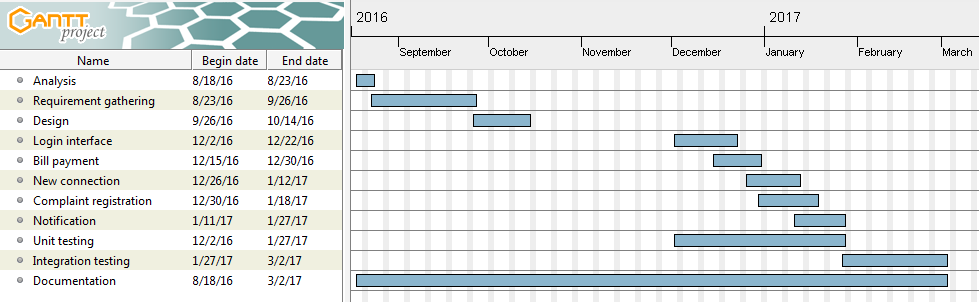
\includegraphics[width=8cm,height=3cm]{newgc.png}
\caption{gantt chart}
\end{figure}
\end{frame}

\begin{frame}
\frametitle{DATA FLOW DIAGRAM}
%\begin{itemize}
%\item LEVEL O DFD
%\includegraphics[width=7cm,height=3cm]{Dfd0.png}
%\end{itemize}
\begin{figure}[center]
\includegraphics[width=6cm,height=5cm]{Dfd0.png}
\caption{LEVEL 0 DFD}
\end{figure}
\end{frame}

\begin{frame}
\frametitle{DATA FLOW DIAGRAM}
%\begin{itemize}
%\item LEVEL 1 DFD
%\includegraphics[width=8cm,height=2cm]{Dfd1.png}
\begin{figure}[center]
\includegraphics[width=10cm,height=4.2cm]{Dfd1.png}
\caption{LEVEL 1 DFD}
\end{figure}
%\end{itemize}
\end{frame}

\begin{frame}
\frametitle{DATA FLOW DIAGRAM}
\begin{figure}[center]
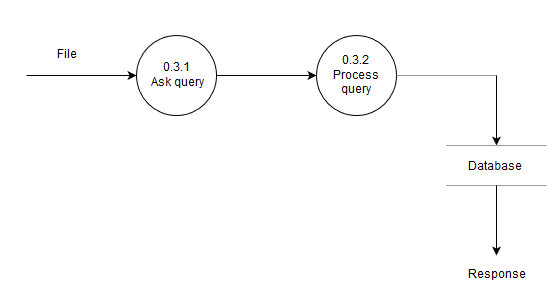
\includegraphics[width=8cm,height=5cm]{Dfd2.png}
\caption{LEVEL 2 DFD}
\end{figure}
\end{frame}


\begin{frame}
\frametitle{USECASE DIAGRAM}
\begin{figure}[center]
\includegraphics[width=4.5cm,height=6cm]{Usecase.png}
%\caption{Usecase Diagram}
\end{figure}
\end{frame}


\begin{frame}
\frametitle{SEQUENCE DIAGRAM}
\begin{figure}[center]
\includegraphics[width=7cm,height=6cm]{sequence.png}
%\caption{Sequence Diagram}
\end{figure}
\end{frame}

\begin{frame}
\frametitle{ACTIVITY DIAGRAM}
\begin{figure}[center]
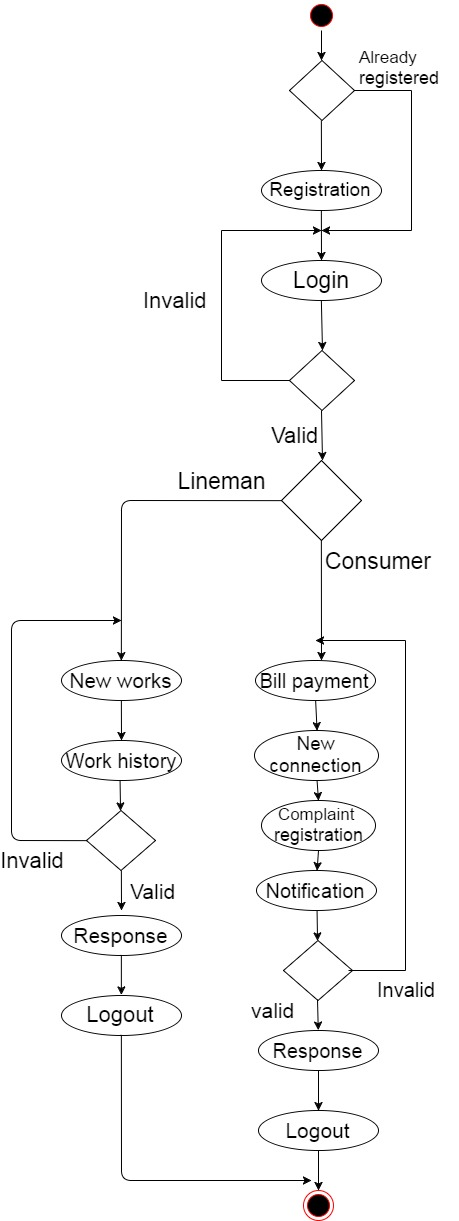
\includegraphics[width=3cm,height=7cm]{activity.jpg}
%\caption{Activity Diagram}
\end{figure}
\end{frame}

\begin{frame}
\frametitle{ER DIAGRAM}
\begin{figure}[center]
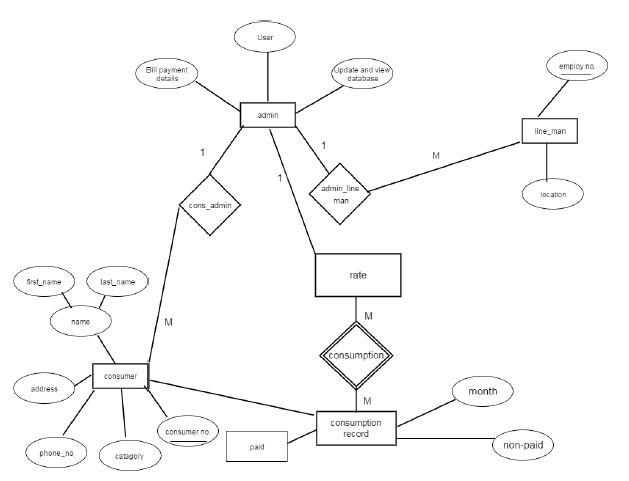
\includegraphics[width=8cm,height=7cm]{err.png}
%\caption{ER Diagram}
\end{figure}
\end{frame}

\begin{frame}
\frametitle{Login Screen}
\begin{figure}[center]
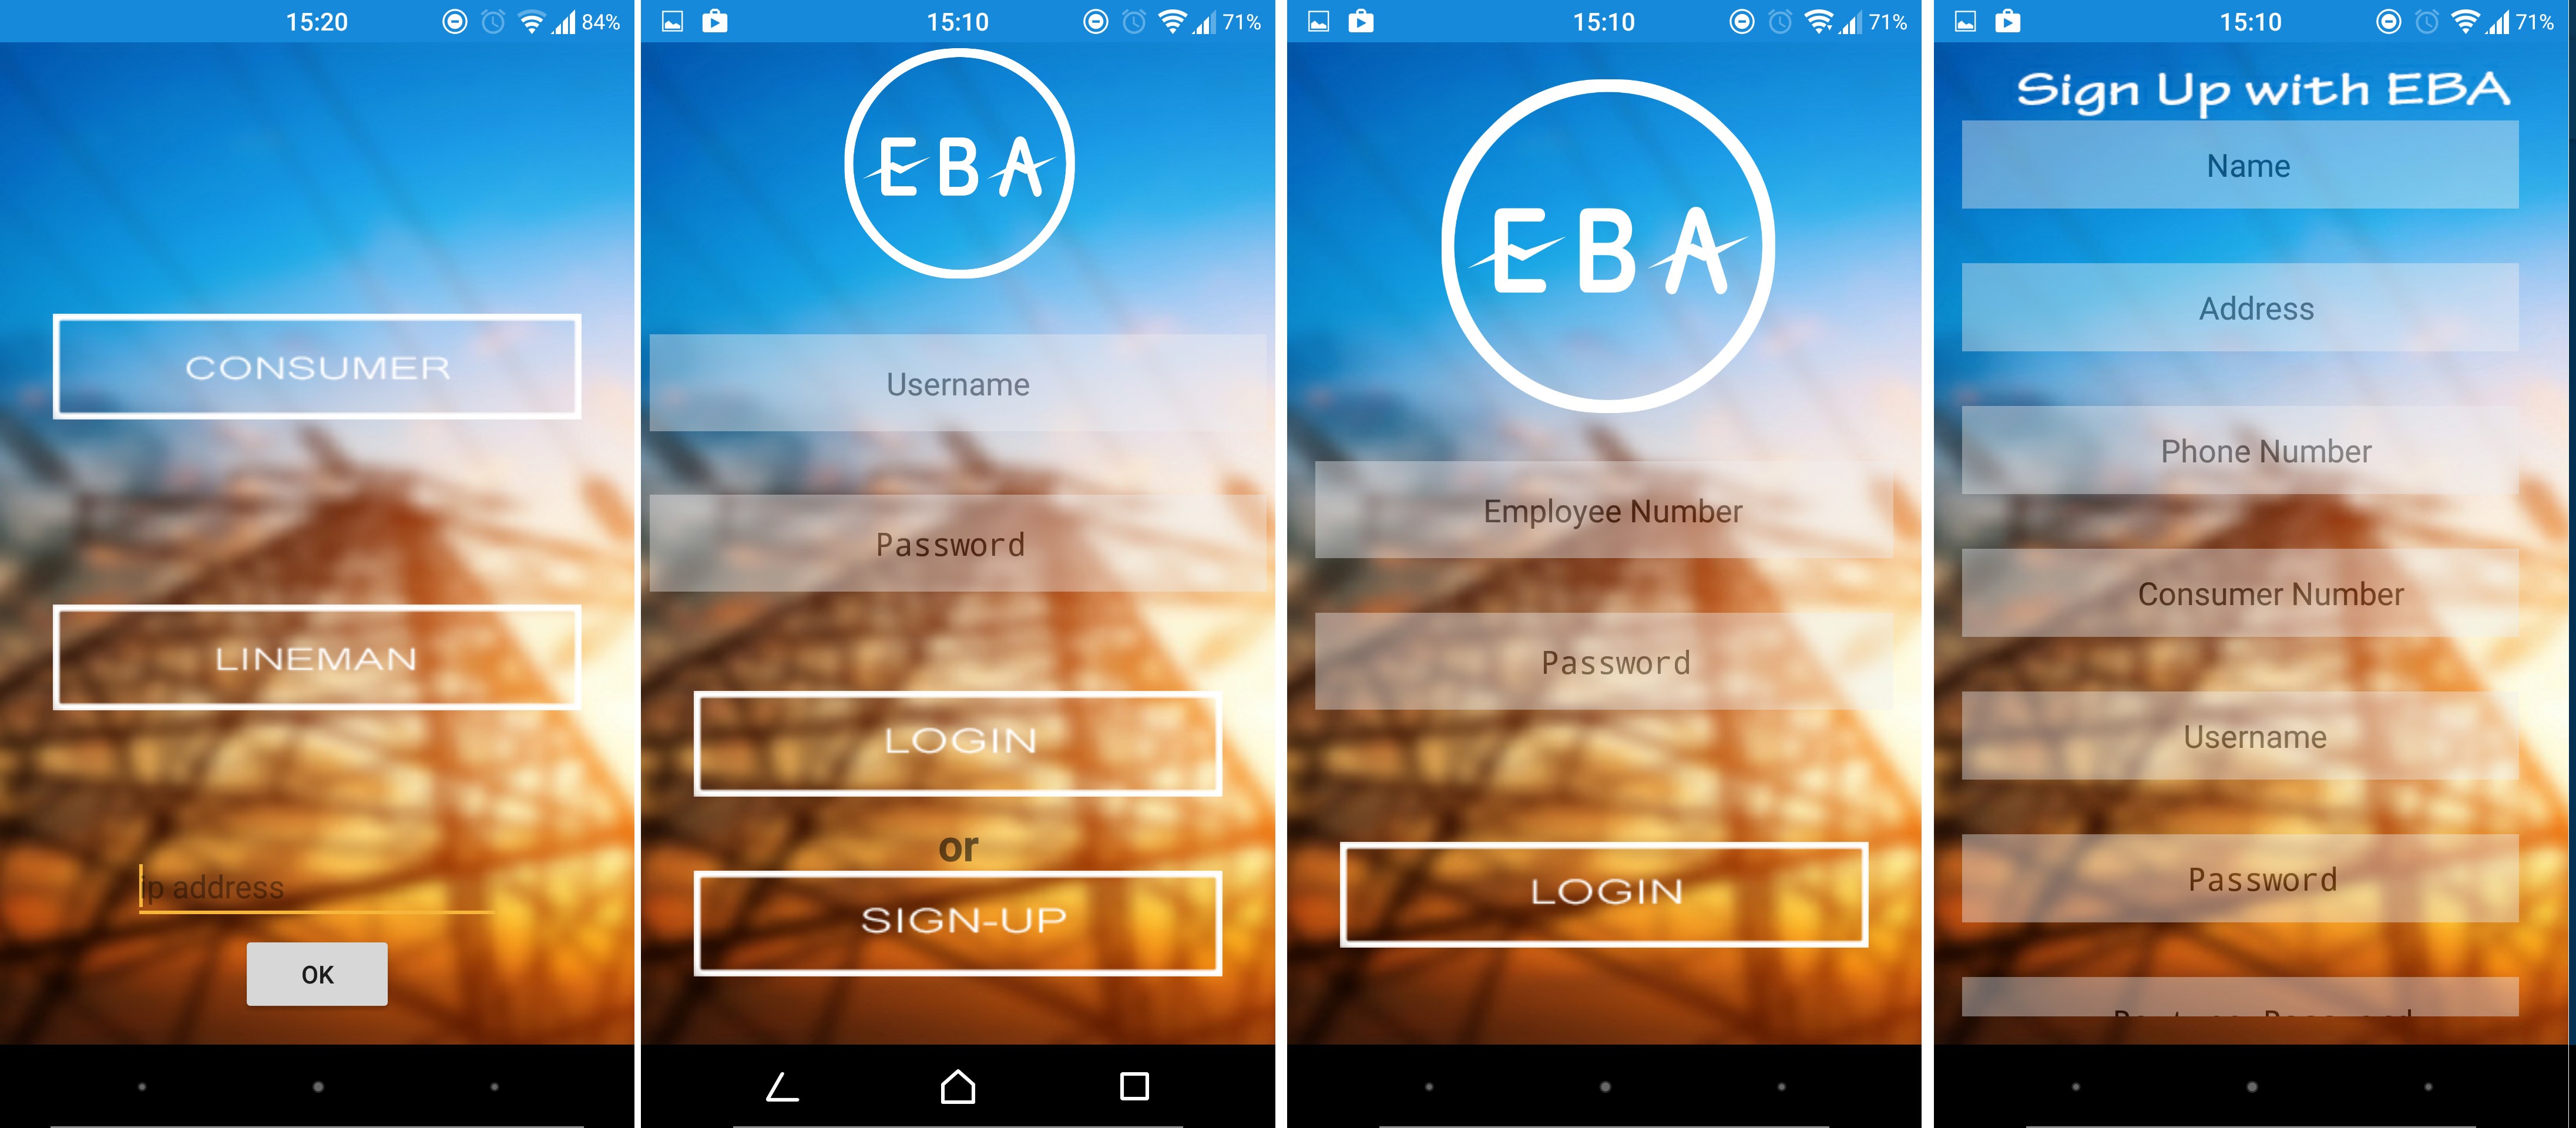
\includegraphics[width=10.1cm ,height=4.5cm]{Loggin.jpg}
%\caption{ER Diagram}
\end{figure}
\end{frame}

\begin{frame}
\frametitle{Home Page}
\begin{figure}[center]
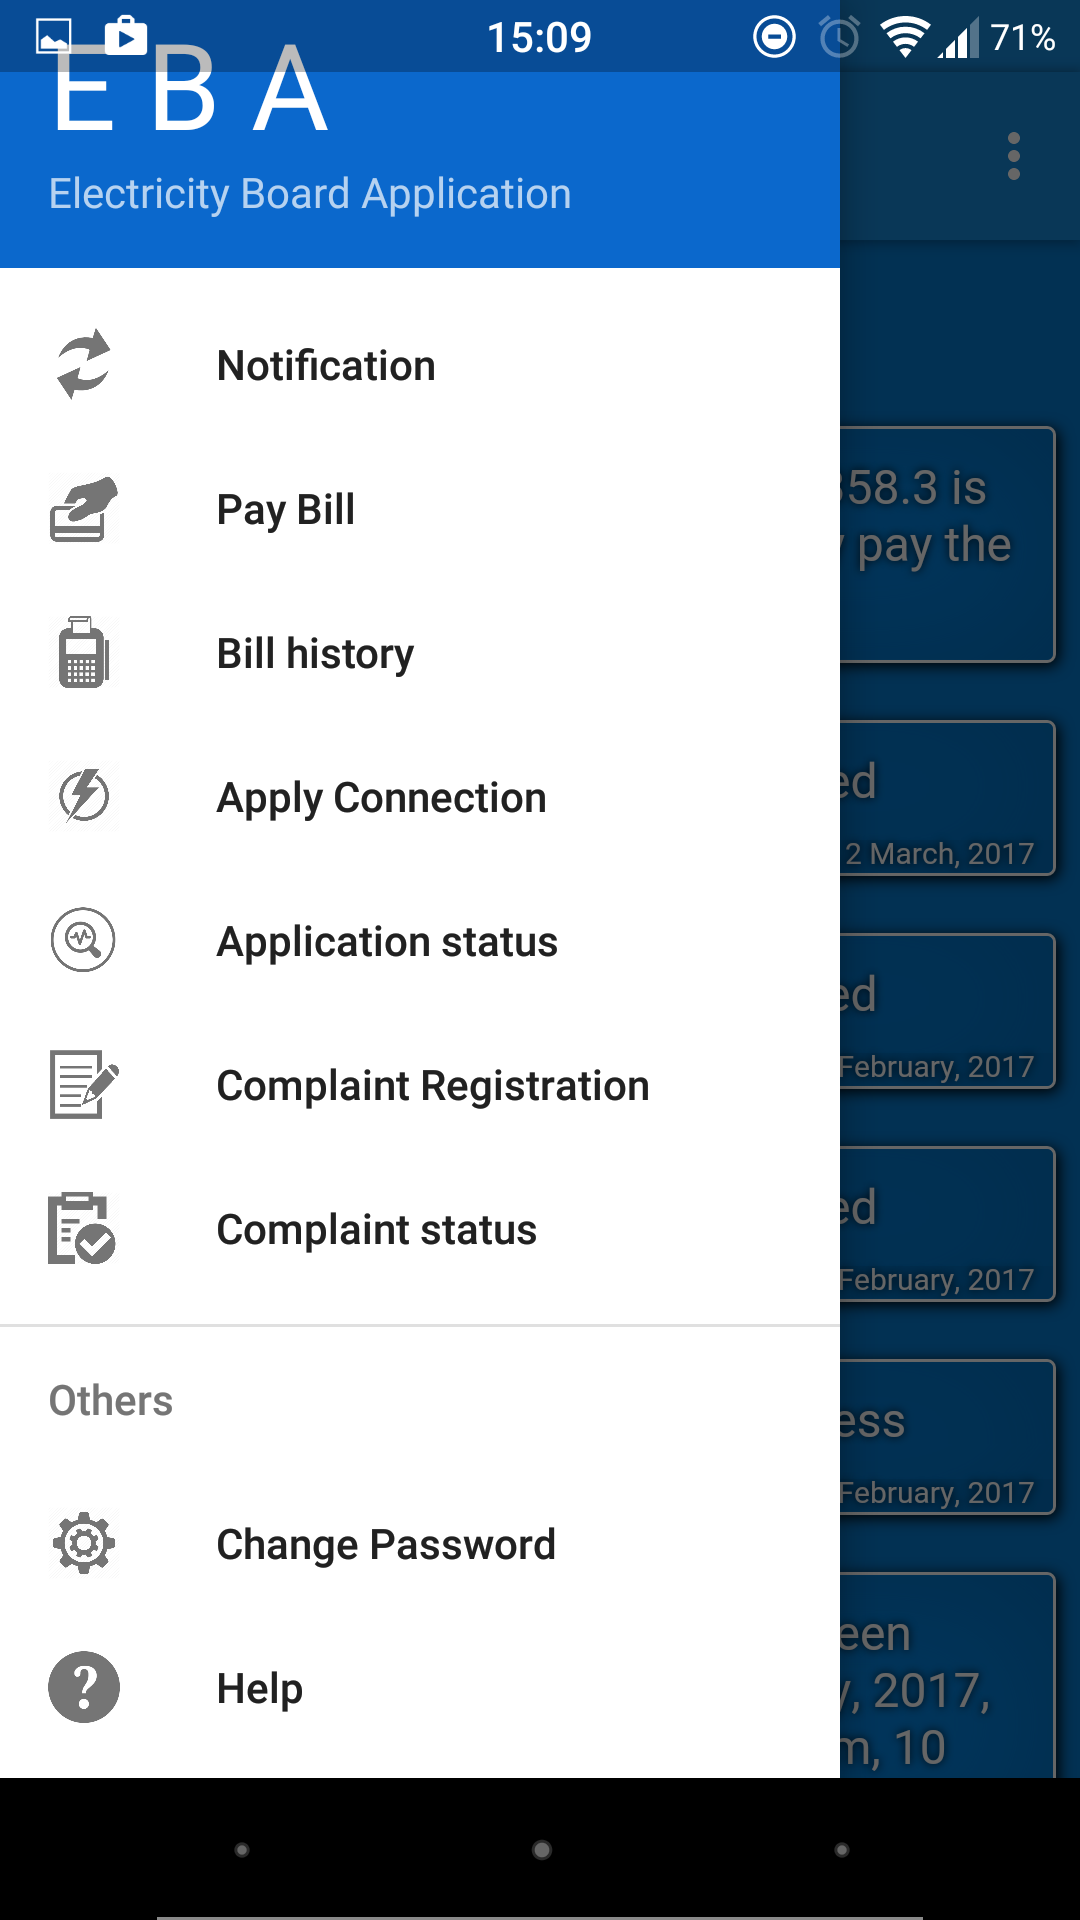
\includegraphics[width=3.4cm ,height=6.3cm]{homepage.png}
\vspace{4cm} 
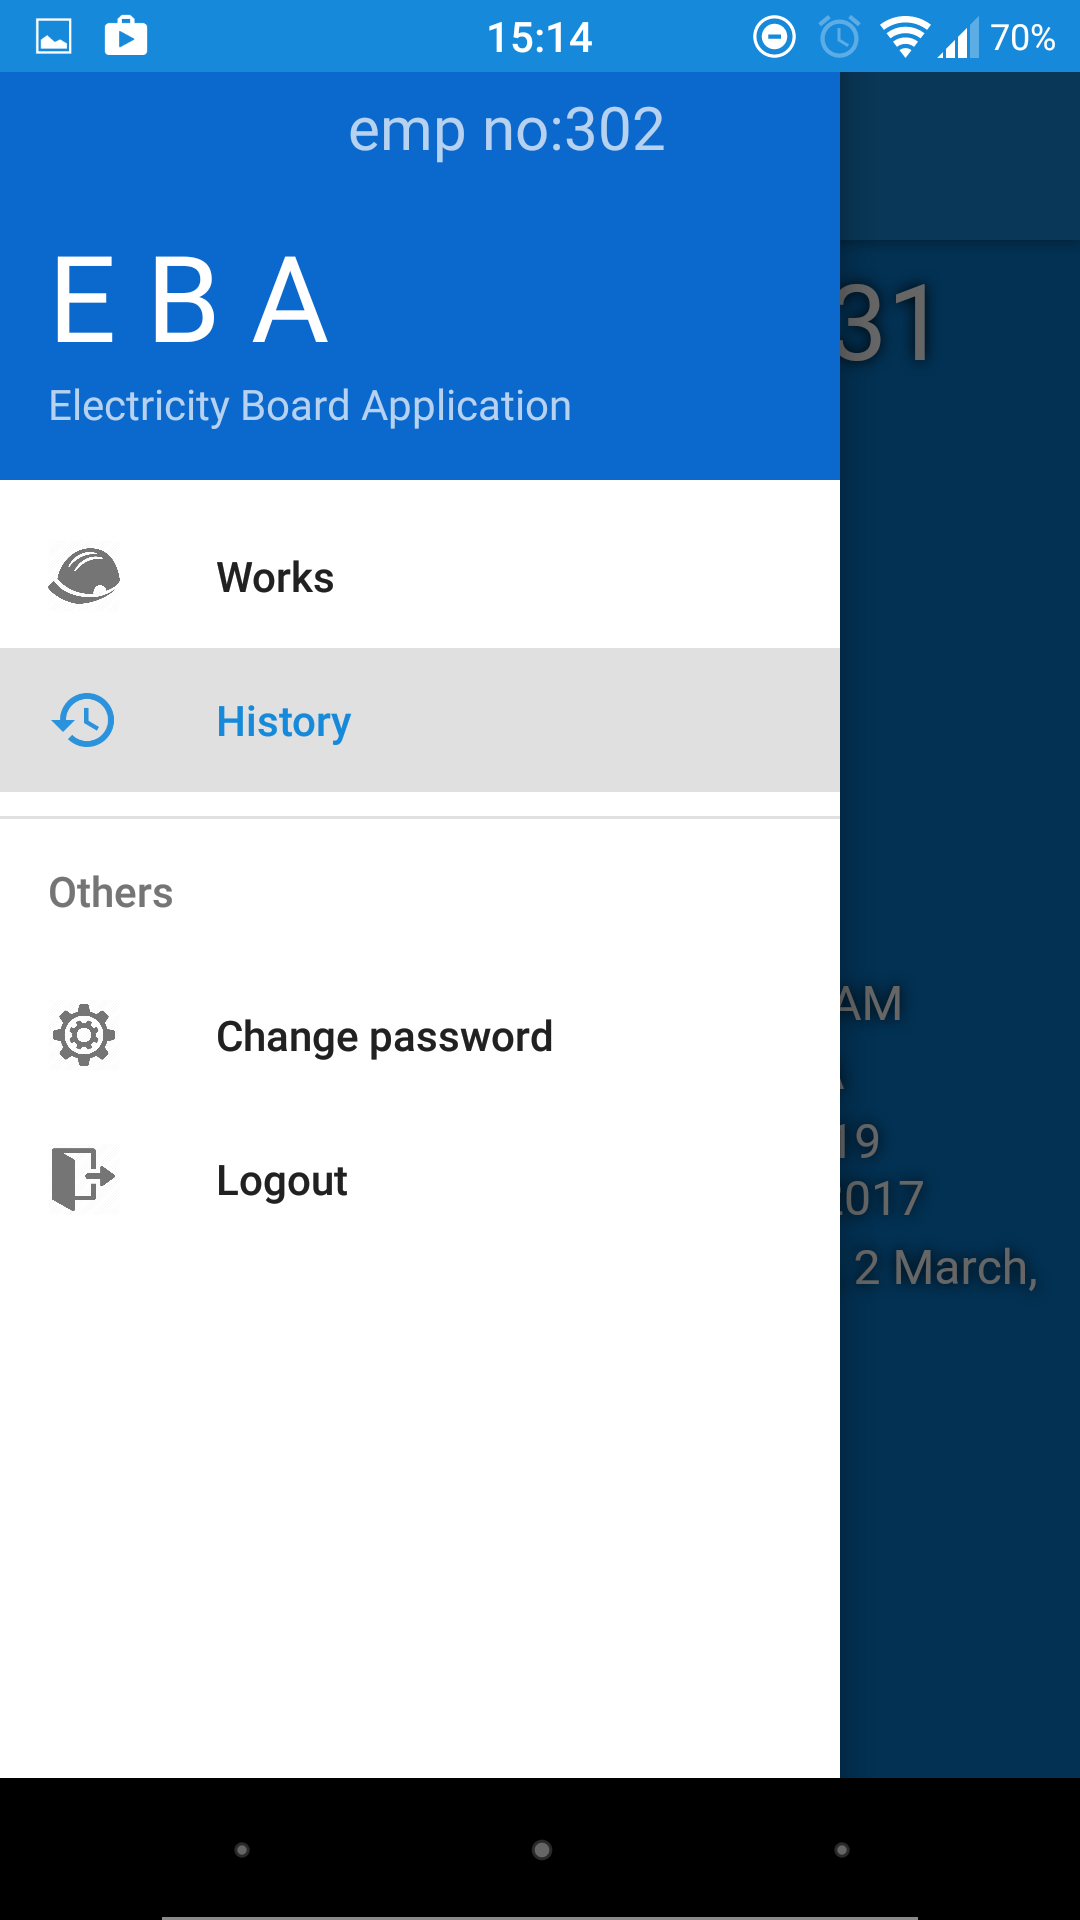
\includegraphics[width=3.4cm ,height=6.3cm]{sslineman.png}
%\caption{ER Diagram}
\end{figure}
\end{frame}

\begin{frame}
\frametitle{User Screen}
\begin{figure}[center]
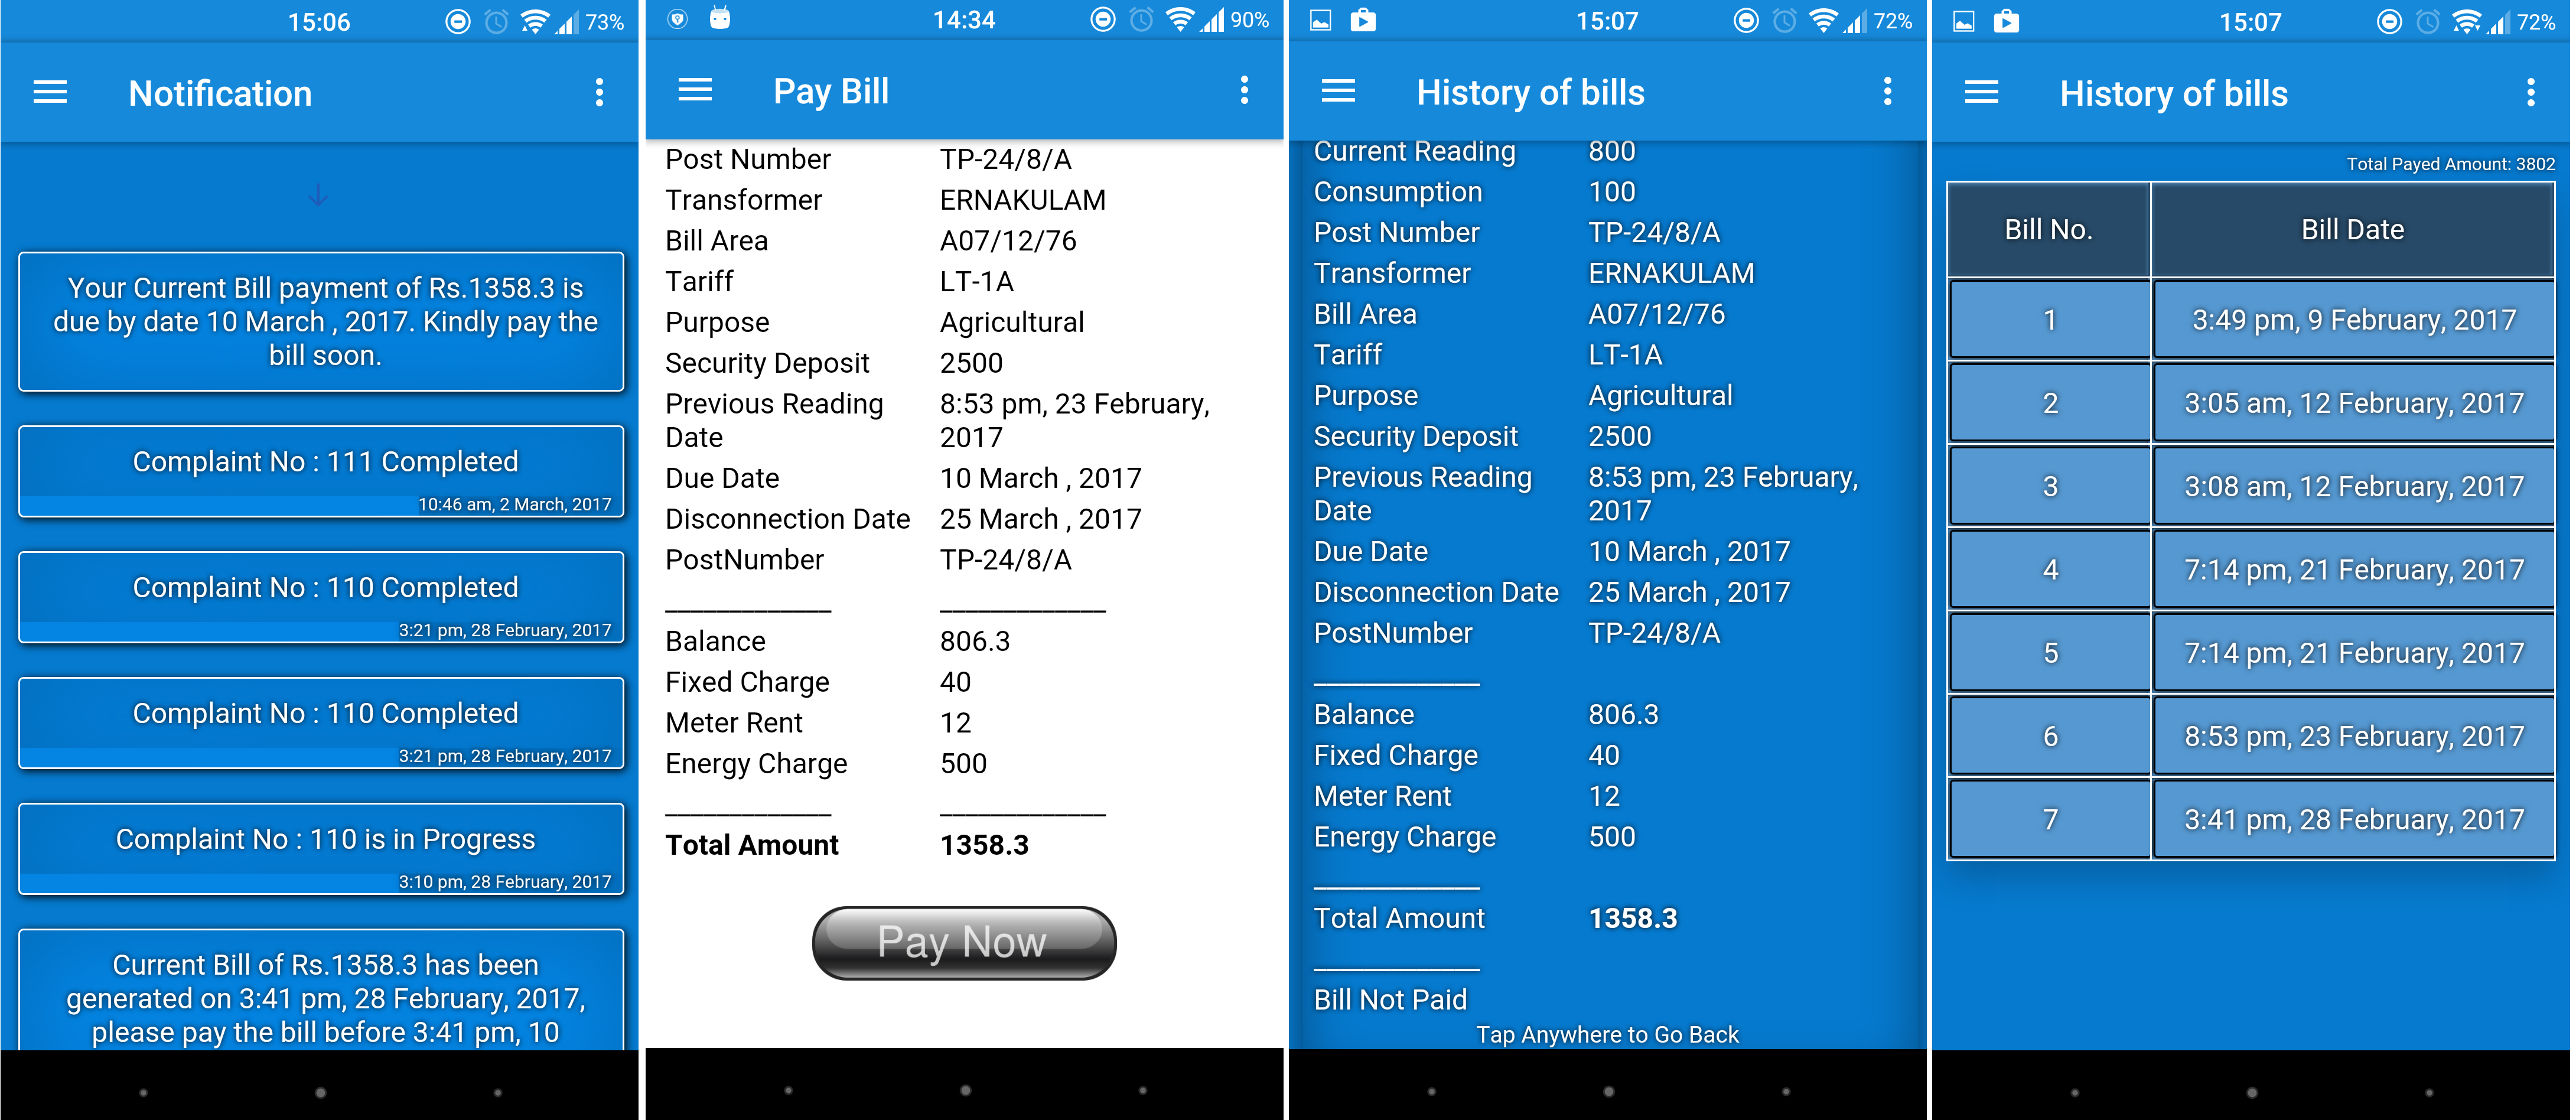
\includegraphics[width=10.1cm ,height=4.5cm]{billhis.jpg} 
%\caption{ER Diagram}
\end{figure}
\end{frame}

\begin{frame}
\frametitle{New Connection And Complaint}
\begin{figure}[center]
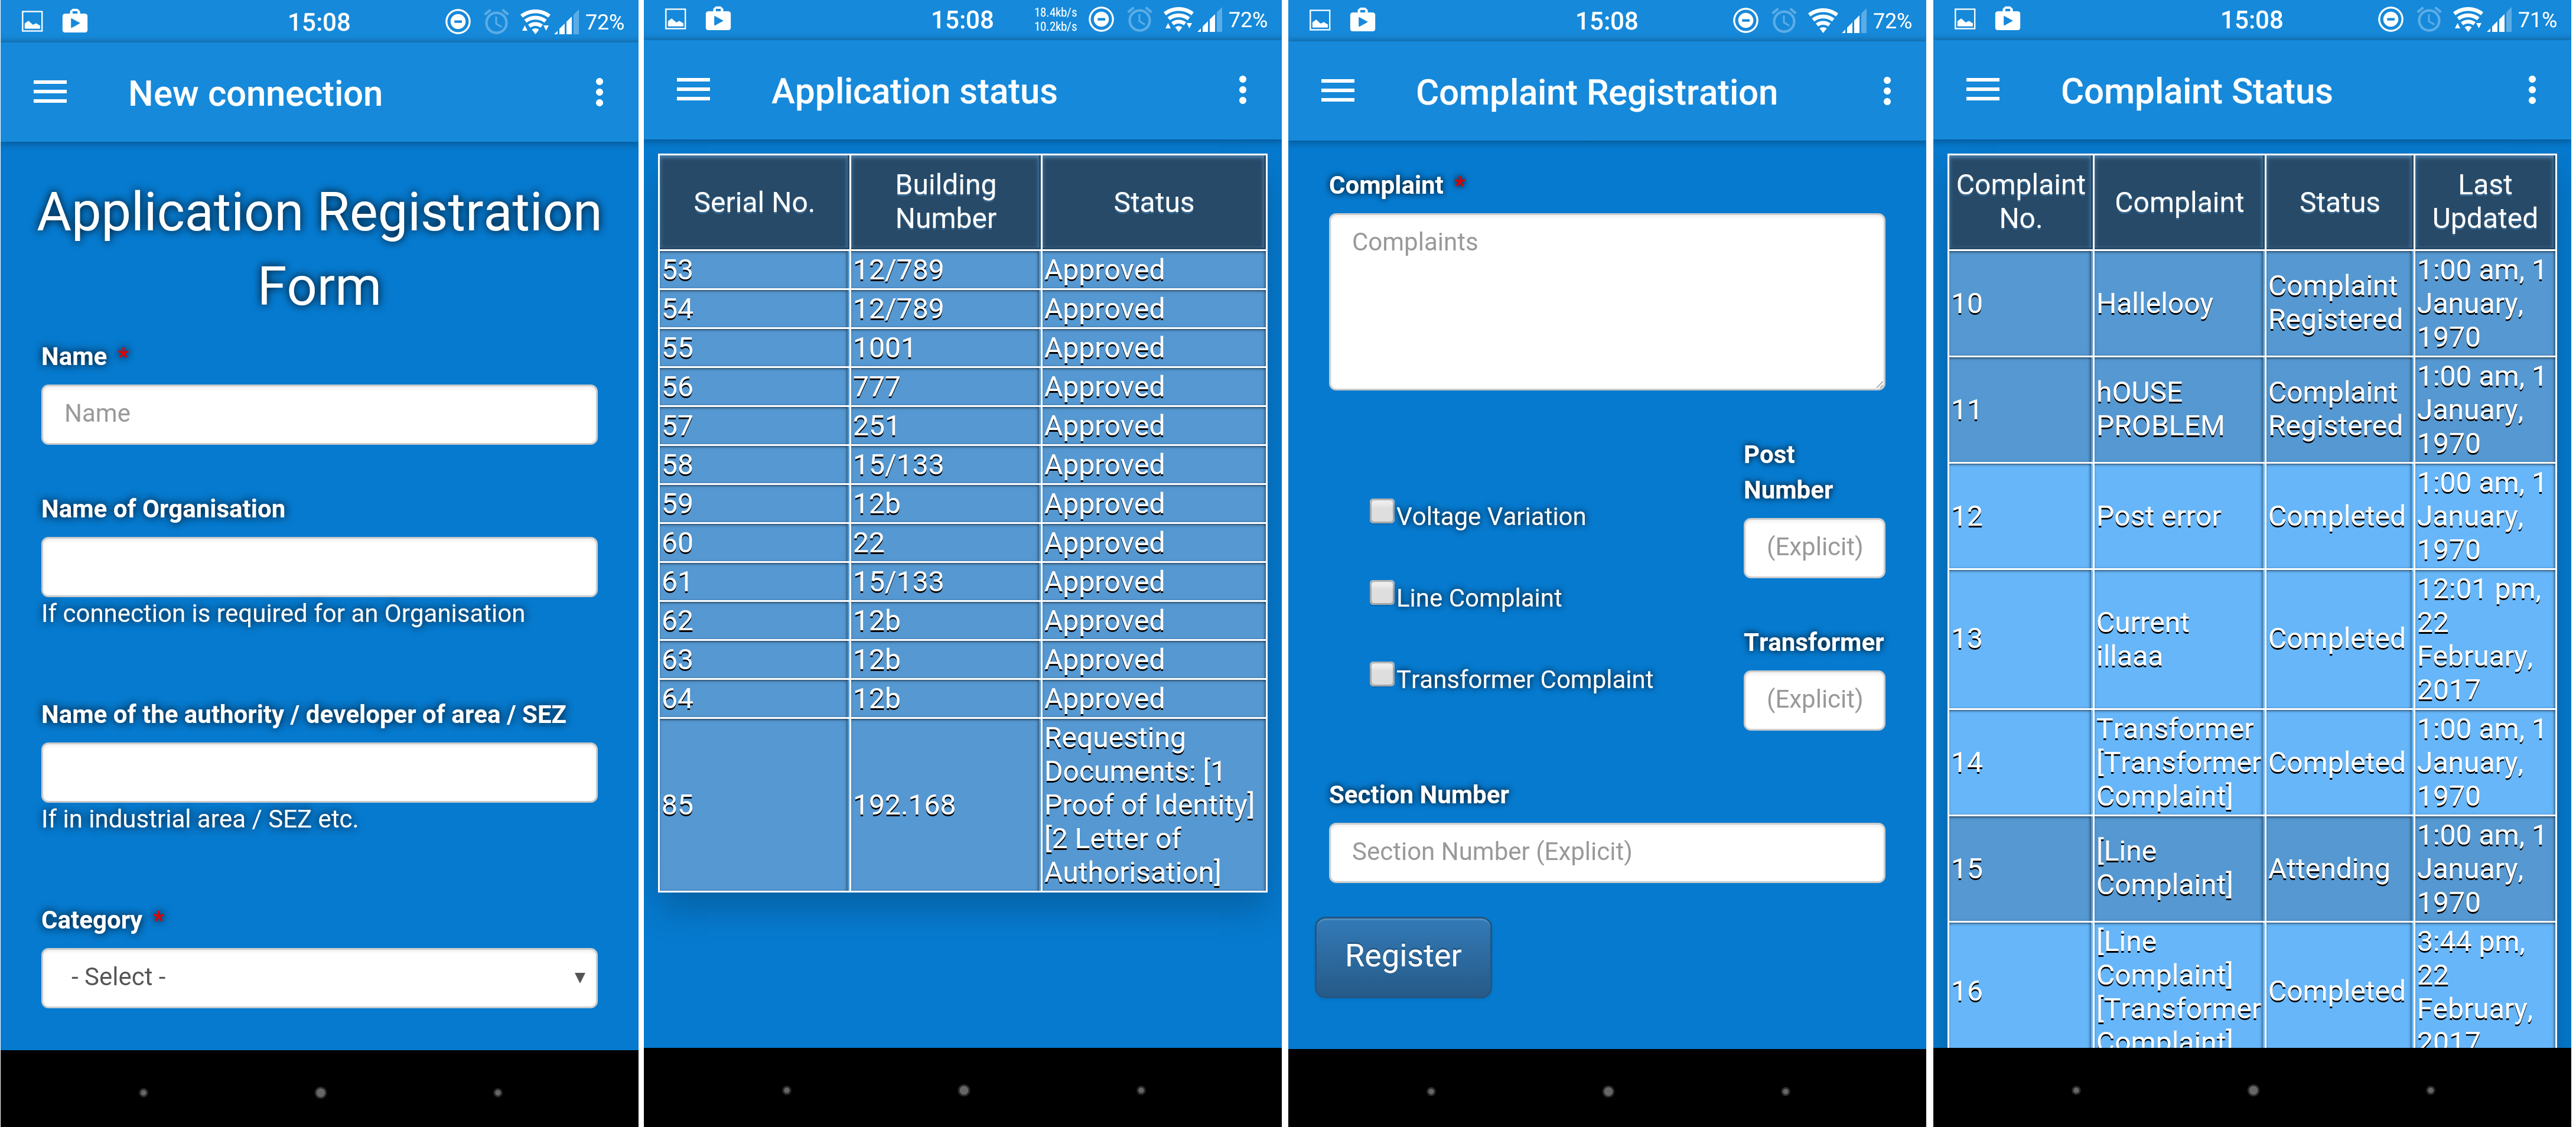
\includegraphics[width=10.1cm ,height=4.5cm]{newcompl.jpg} 
%\caption{ER Diagram}
\end{figure}
\end{frame}

\begin{frame}
\frametitle{Lineman View}
\begin{figure}[center]
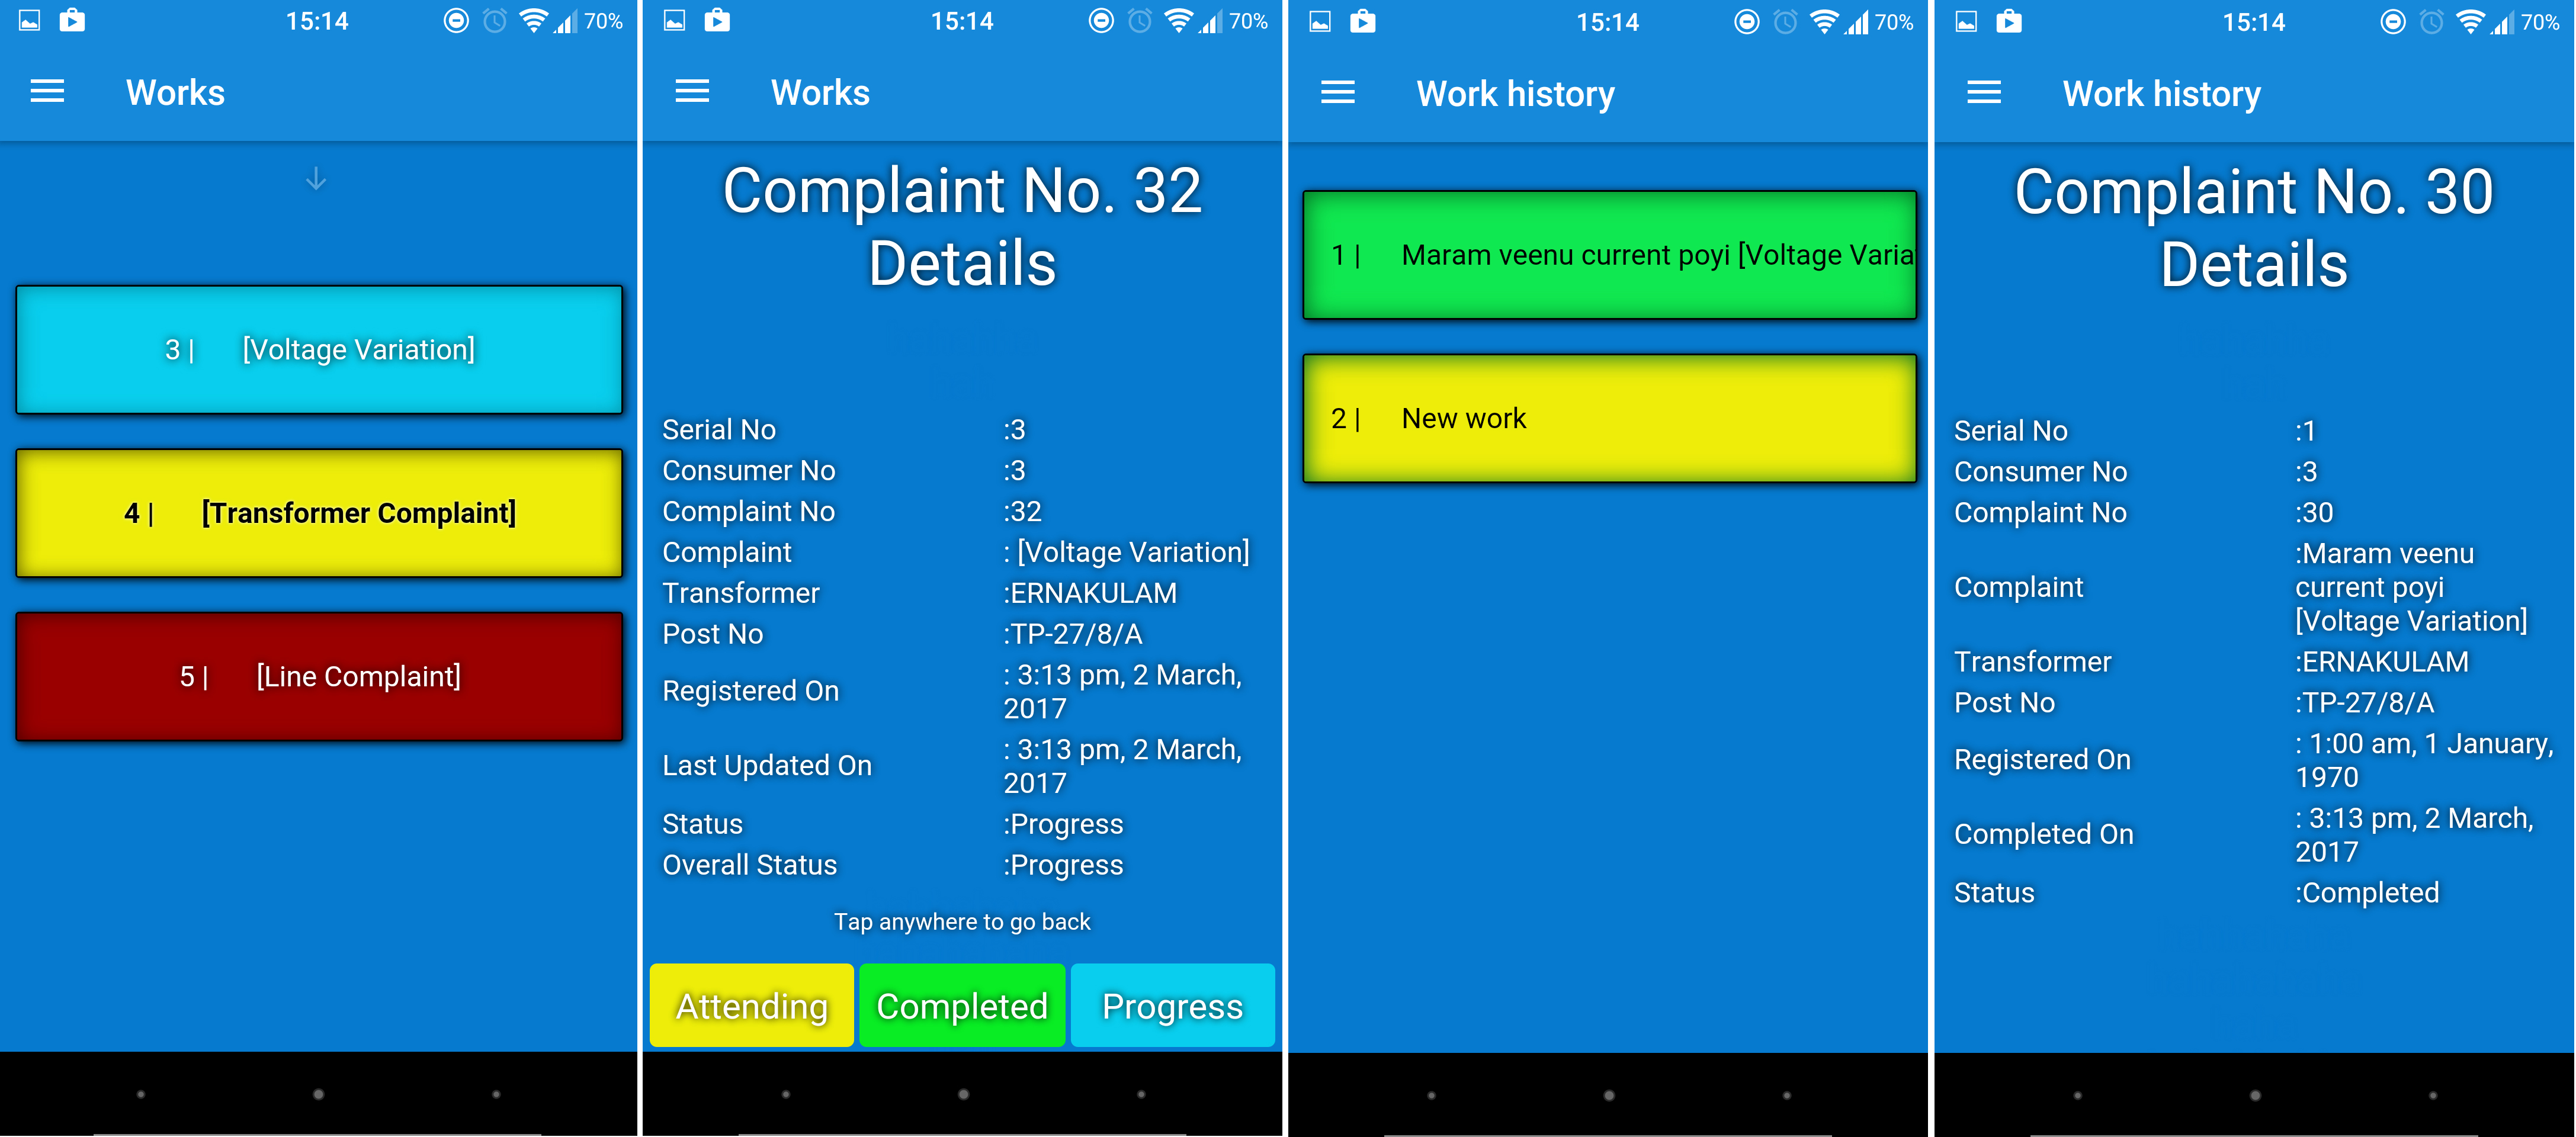
\includegraphics[width=10.1cm ,height=4.5cm]{linehome.jpg} 
%\caption{ER Diagram}
\end{figure}
\end{frame}

\begin{frame}
\frametitle{Settings And Help}
\begin{figure}[center]
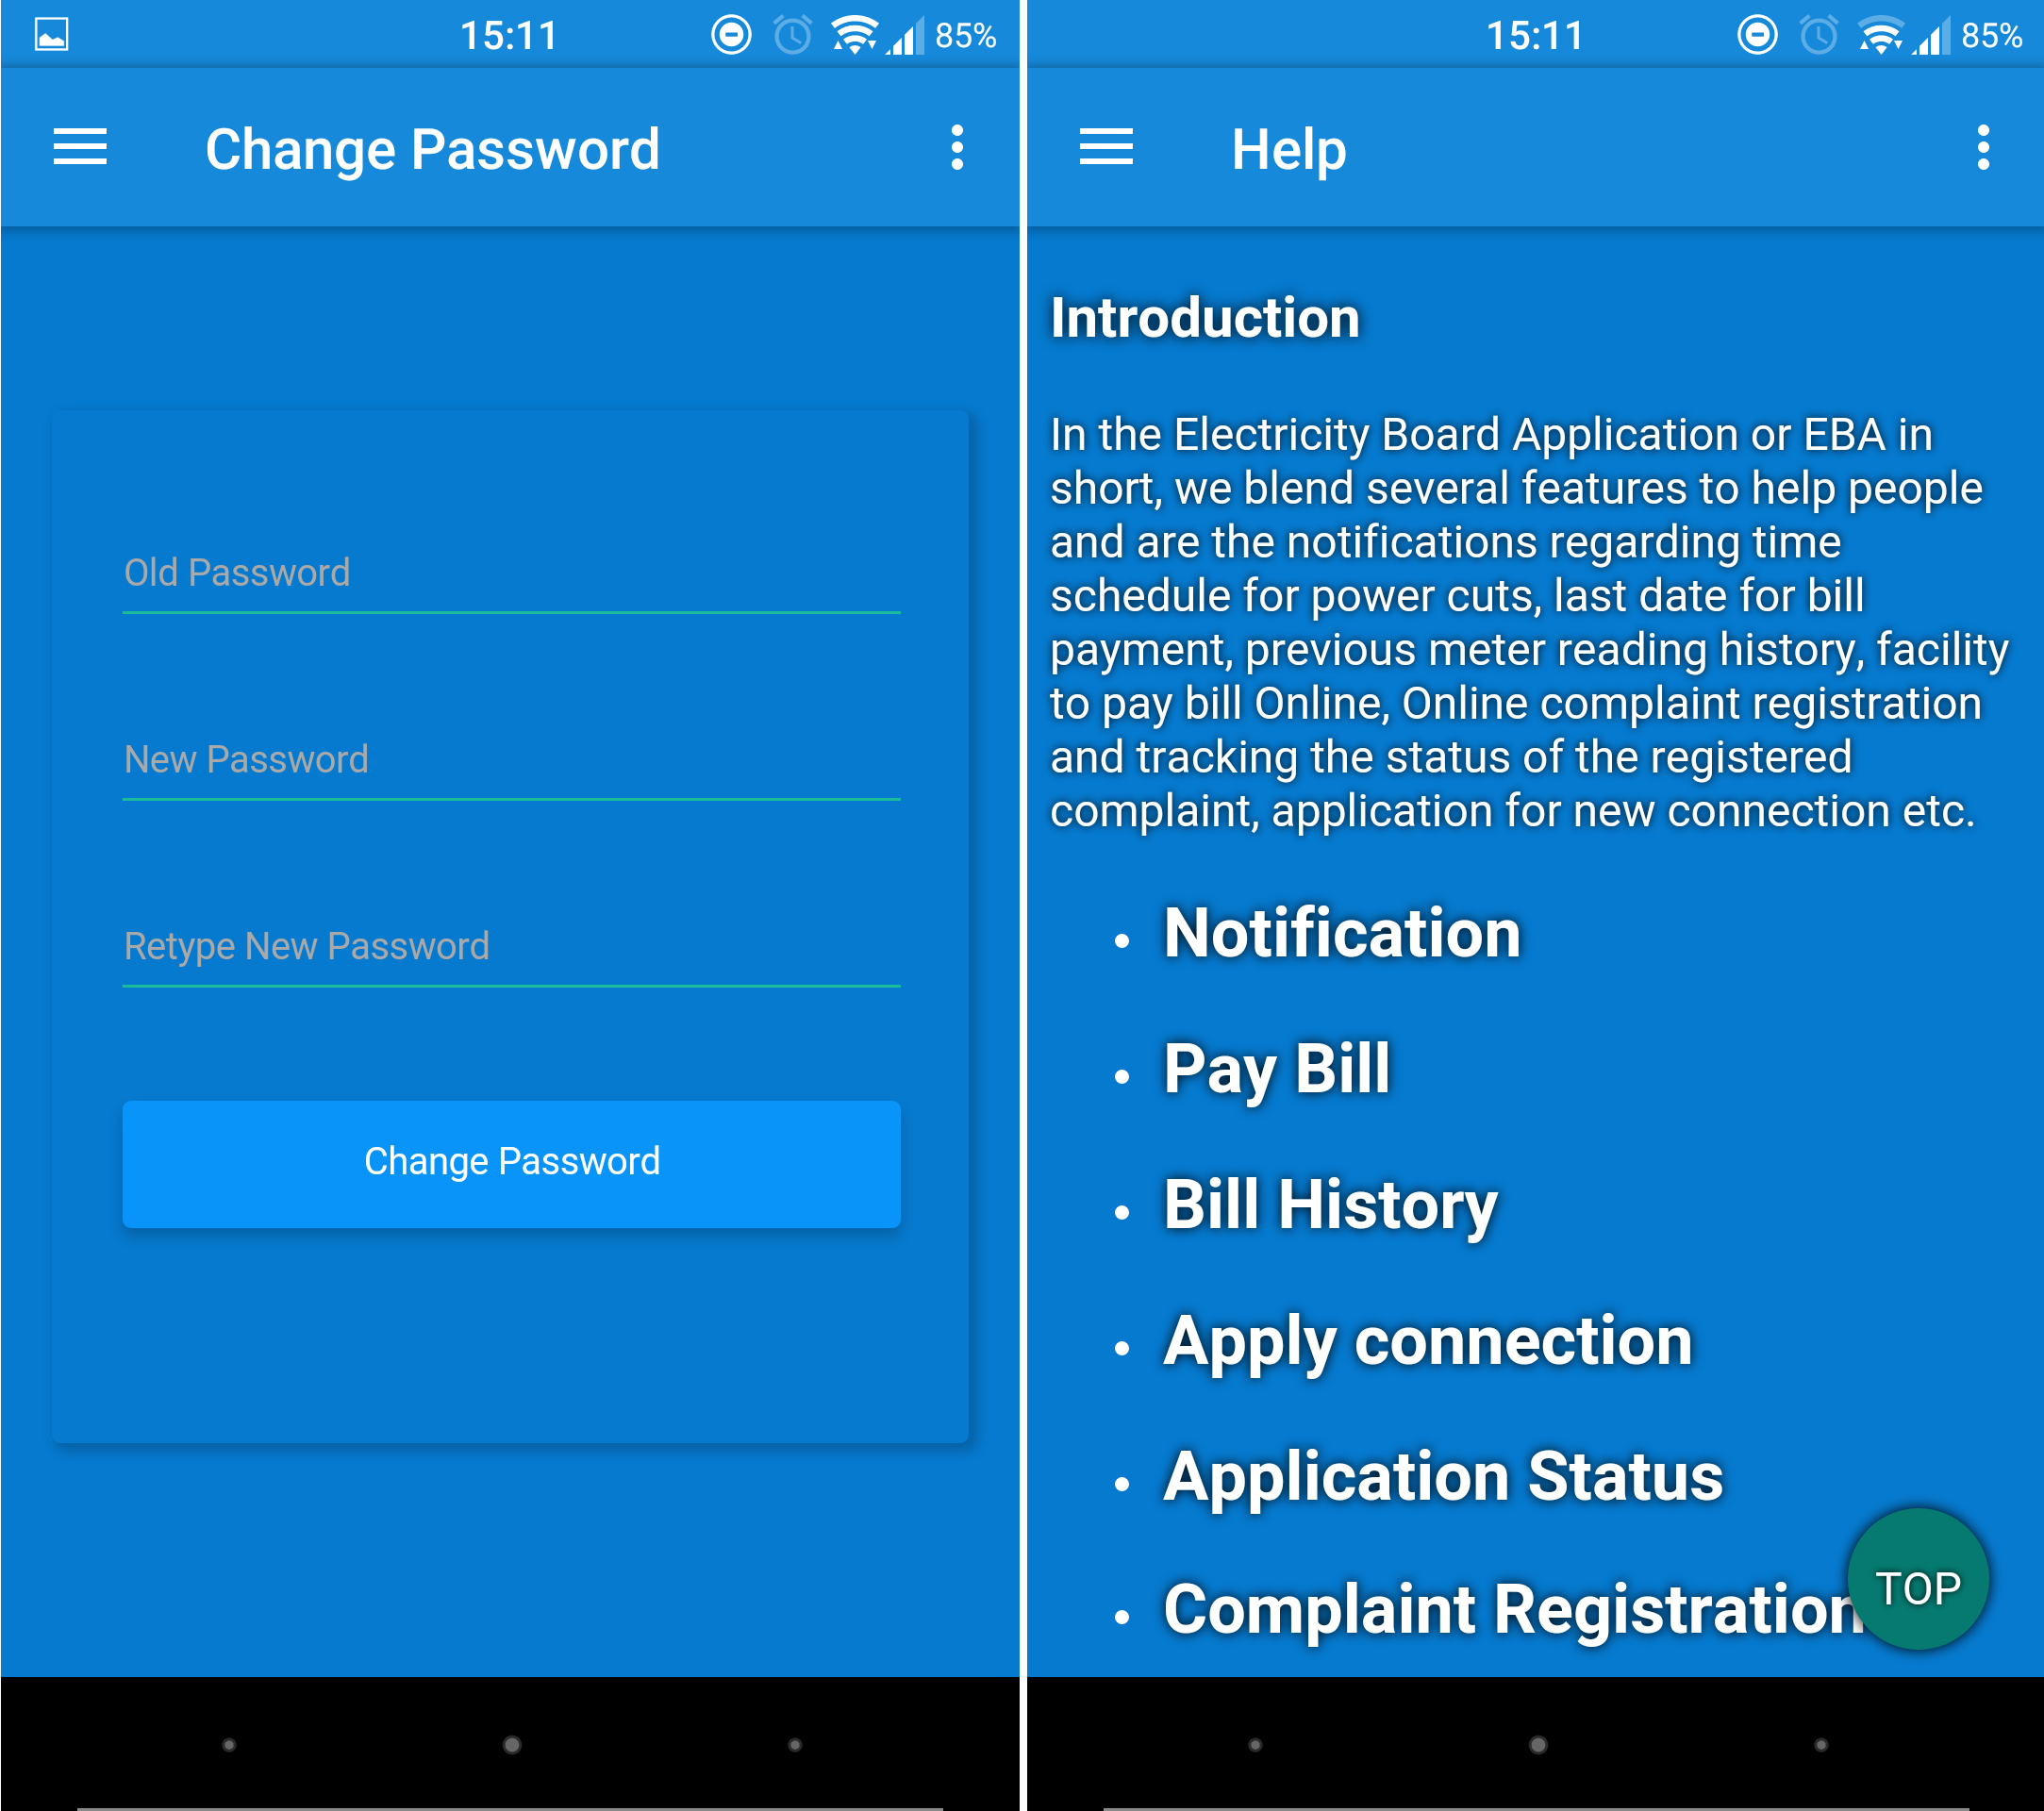
\includegraphics[width=7cm ,height=6.4cm]{helppass.jpg} 
%\caption{ER Diagram}
\end{figure}
\end{frame}

\begin{frame}
\frametitle{Admin Login}
\begin{figure}[center]
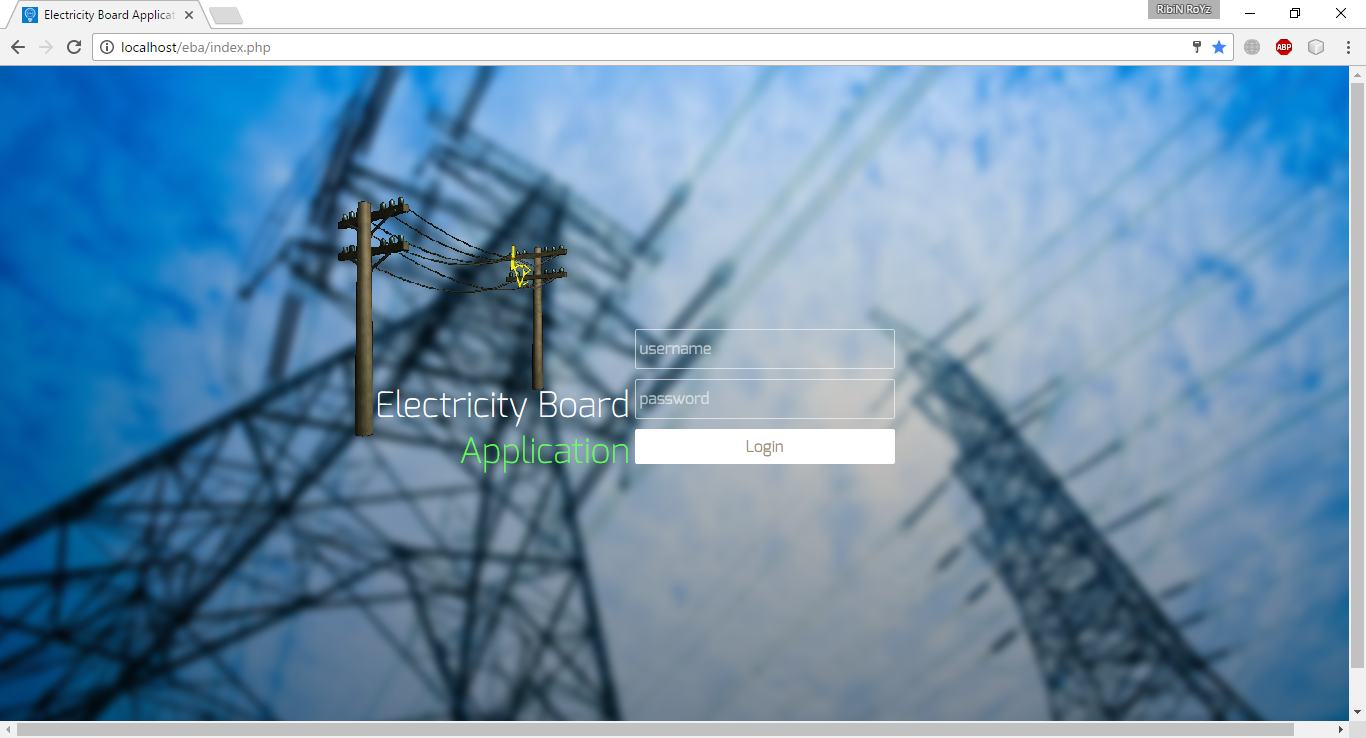
\includegraphics[width=10cm ,height=5.9cm]{index.png} 
%\caption{ER Diagram}
\end{figure}
\end{frame}


\begin{frame}
\frametitle{Home Page}
\begin{figure}[center]
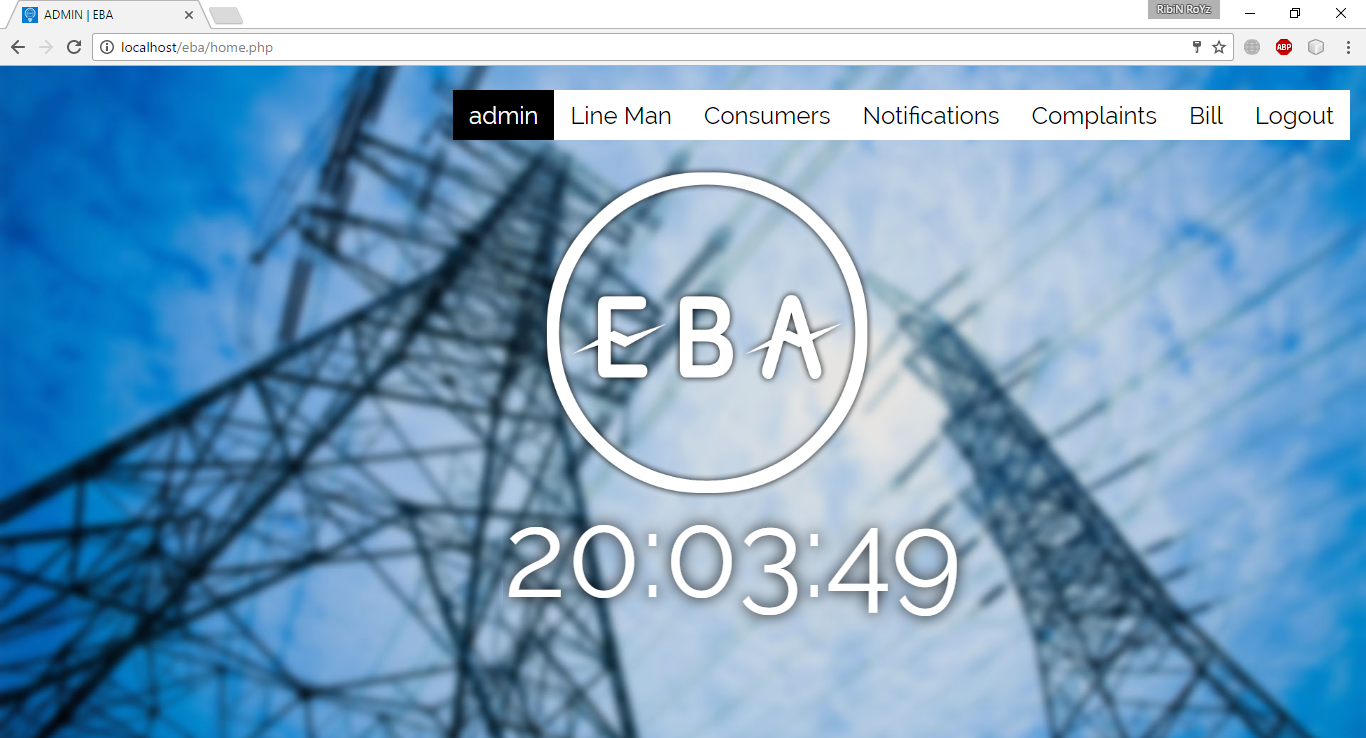
\includegraphics[width=10cm ,height=5.9cm]{loggedin.png} 
%\caption{ER Diagram}
\end{figure}
\end{frame}

\begin{frame}
\frametitle{Line Man Add}
\begin{figure}[center]
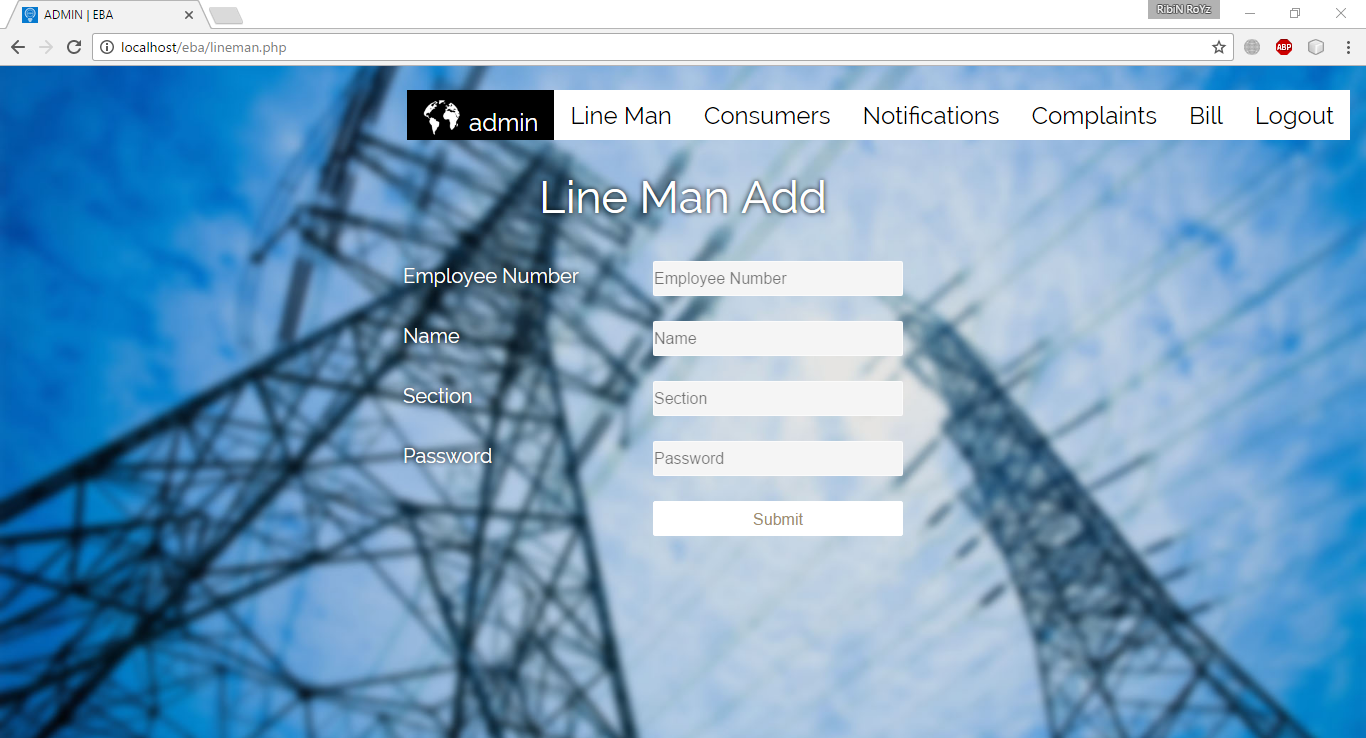
\includegraphics[width=10cm ,height=5.9cm]{linemanadd.png} 
%\caption{ER Diagram}
\end{figure}
\end{frame}

\begin{frame}
\frametitle{Line Man View}
\begin{figure}[center]
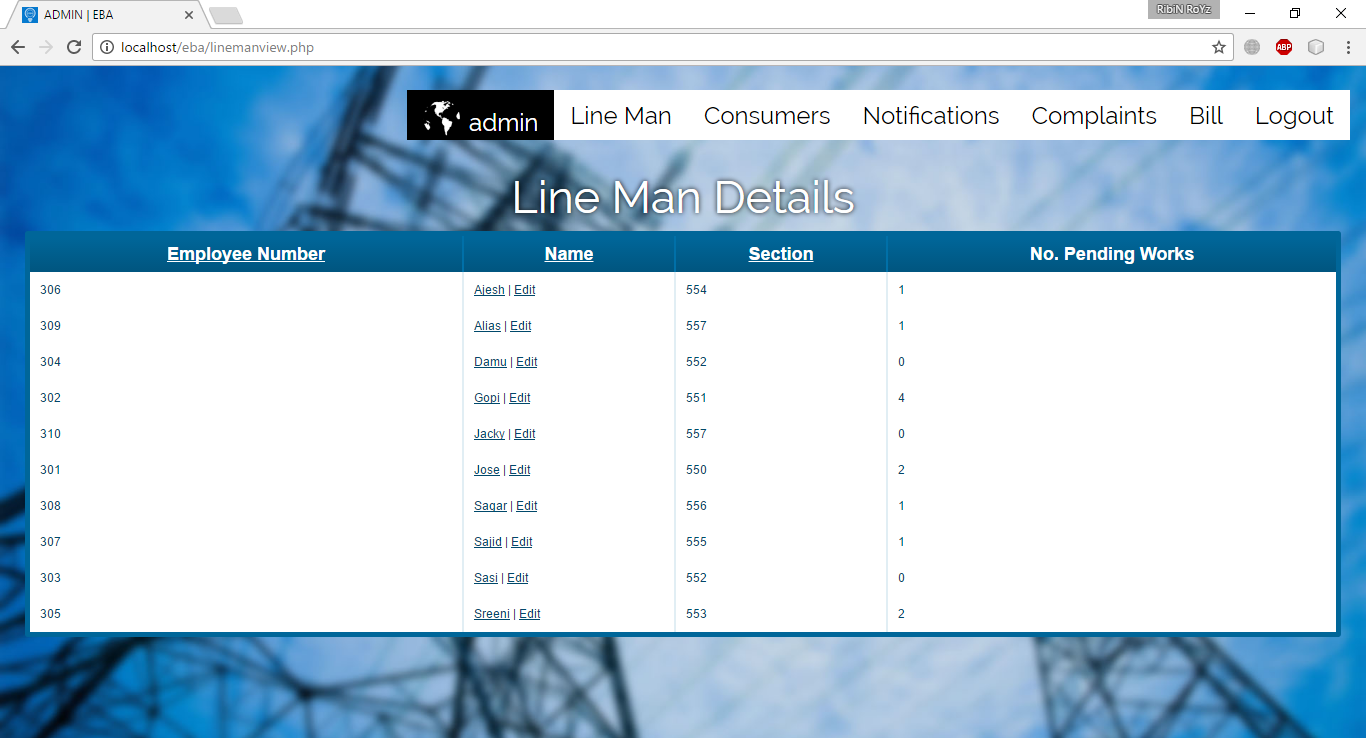
\includegraphics[width=10cm ,height=5.9cm]{linemanview.png} 
%\caption{ER Diagram}
\end{figure}
\end{frame}

\begin{frame}
\frametitle{Line Man Edit }
\begin{figure}[center]
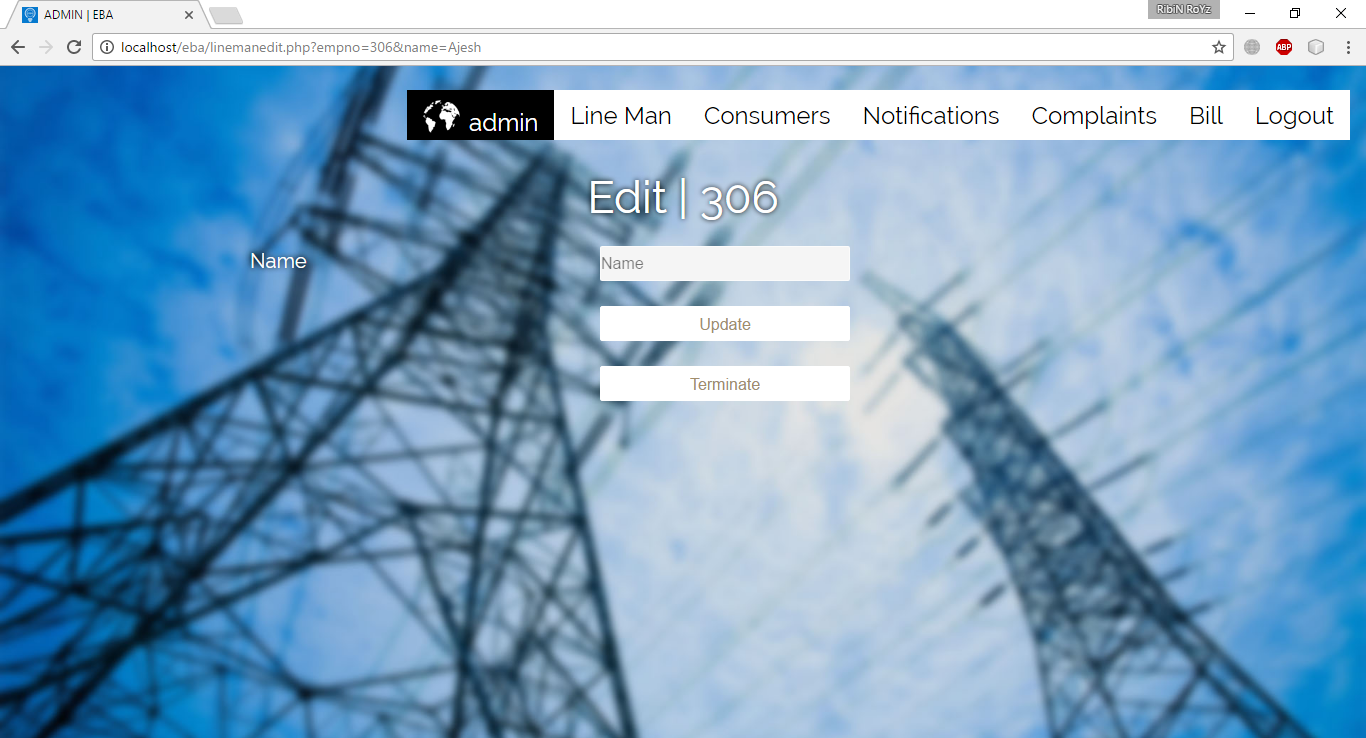
\includegraphics[width=10cm ,height=5.9cm]{linemanedit.png} 
%\caption{ER Diagram}
\end{figure}
\end{frame}

\begin{frame}
\frametitle{Line Man View Detail}
\begin{figure}[center]
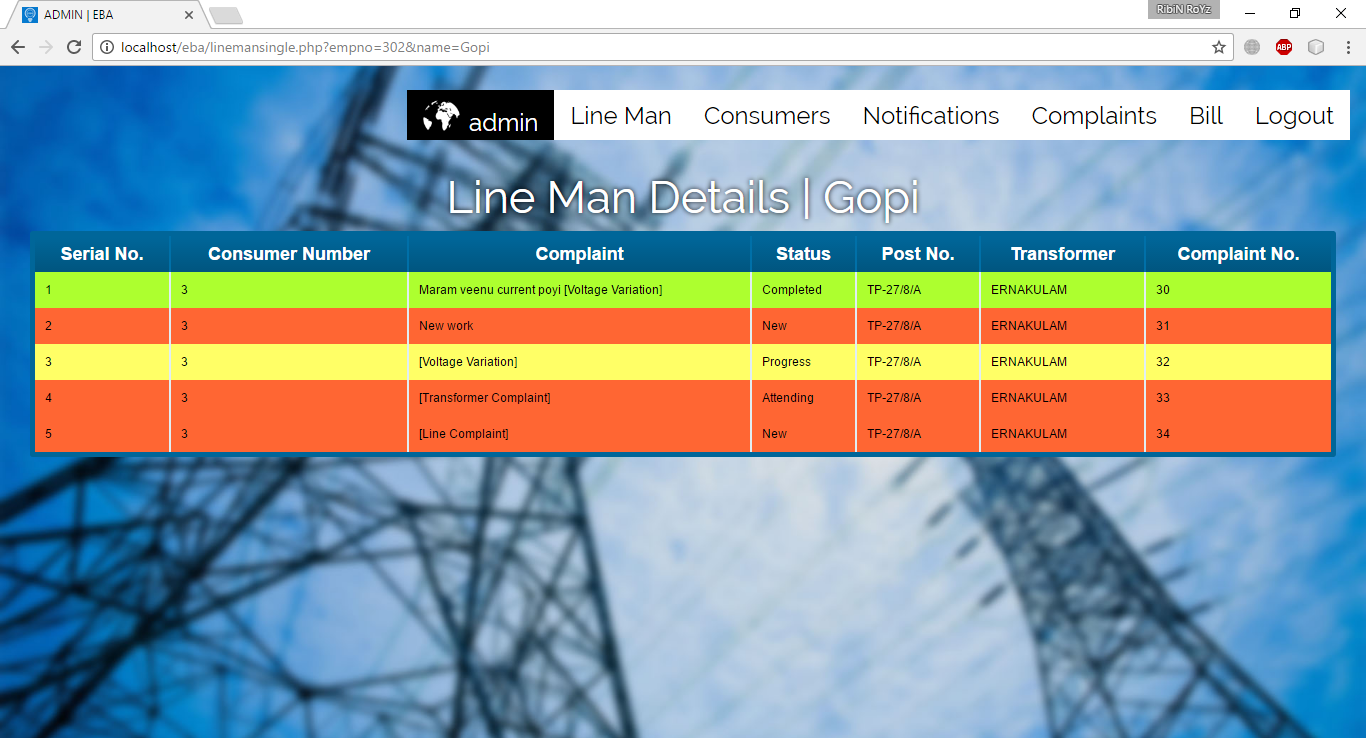
\includegraphics[width=10cm ,height=5.9cm]{linemanviewdetail.png} 
%\caption{ER Diagram}
\end{figure}
\end{frame}

\begin{frame}
\frametitle{Verification }
\begin{figure}[center]
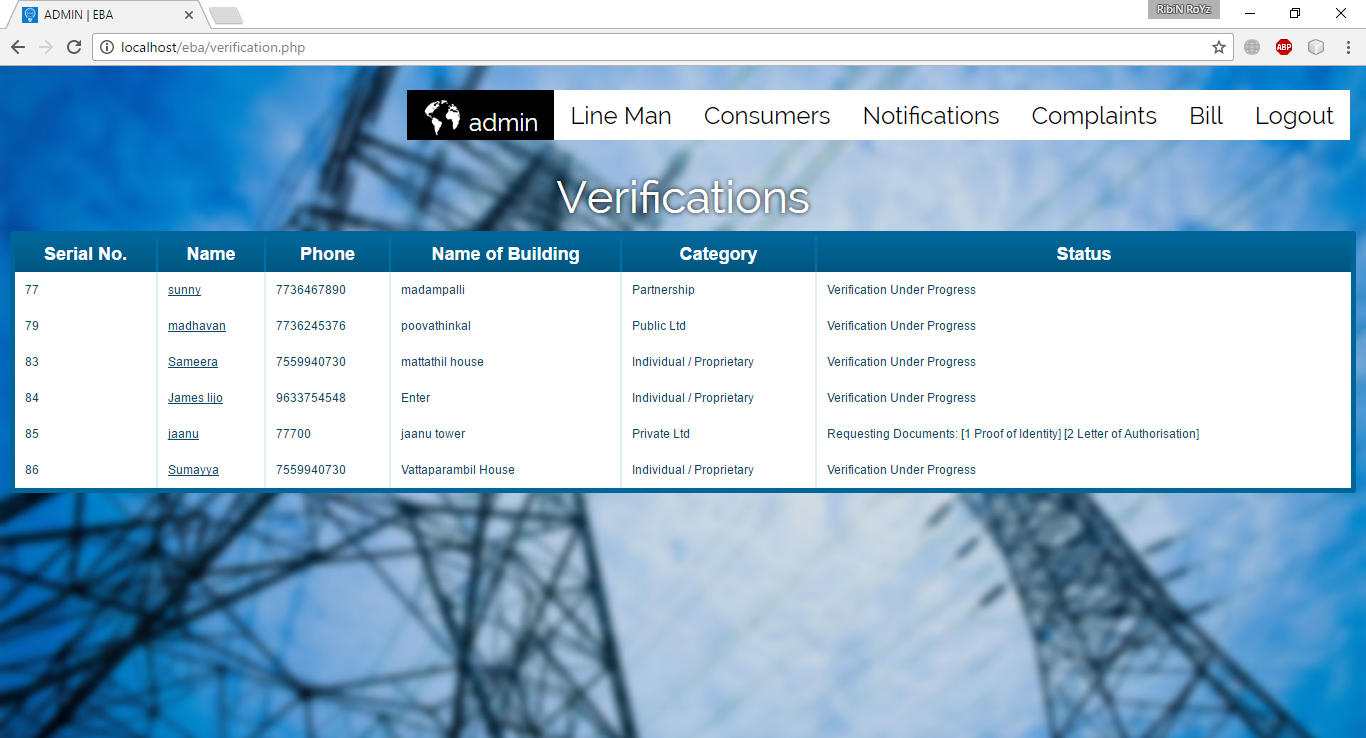
\includegraphics[width=10cm ,height=5.9cm]{verification.png} 
%\caption{ER Diagram}
\end{figure}
\end{frame}

\begin{frame}
\frametitle{Verify Single }
\begin{figure}[center]
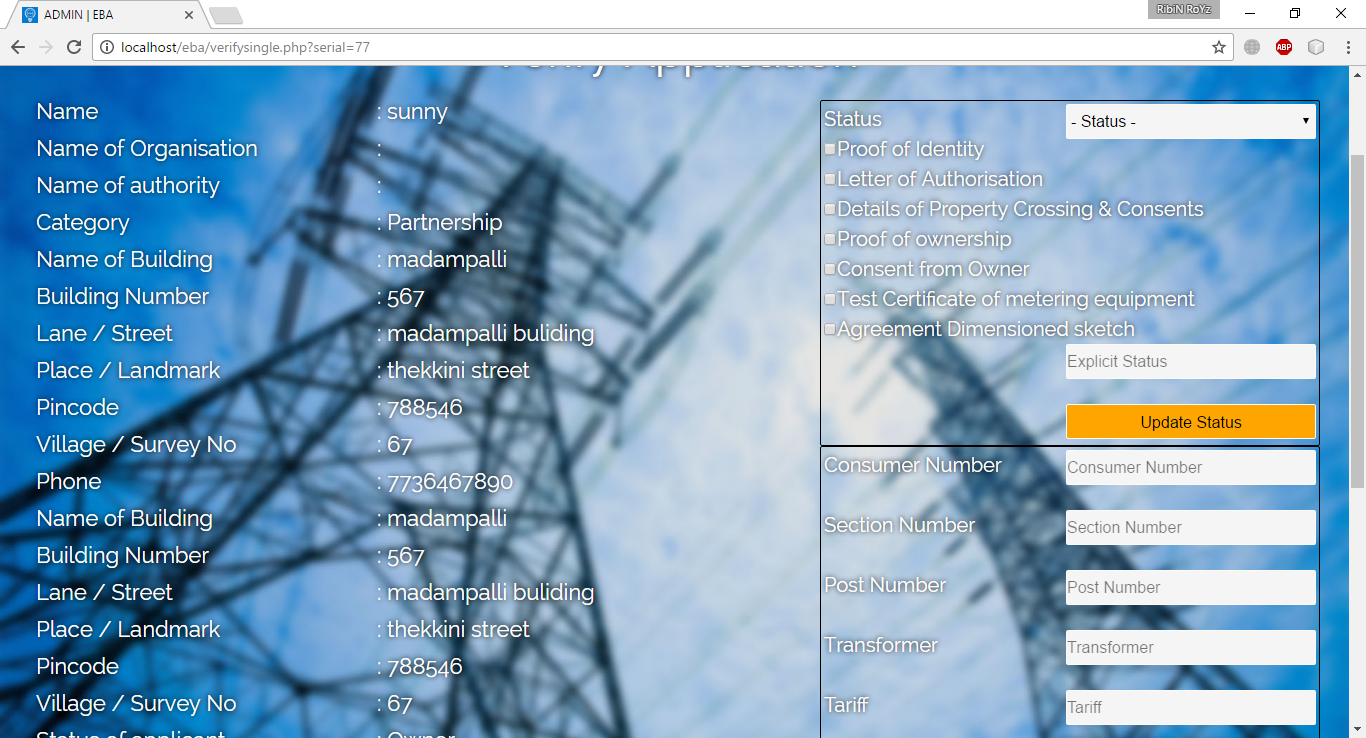
\includegraphics[width=10cm ,height=5.9cm]{verifysingle.png} 
%\caption{ER Diagram}
\end{figure}
\end{frame}

\begin{frame}
\frametitle{EBA Users}
\begin{figure}[center]
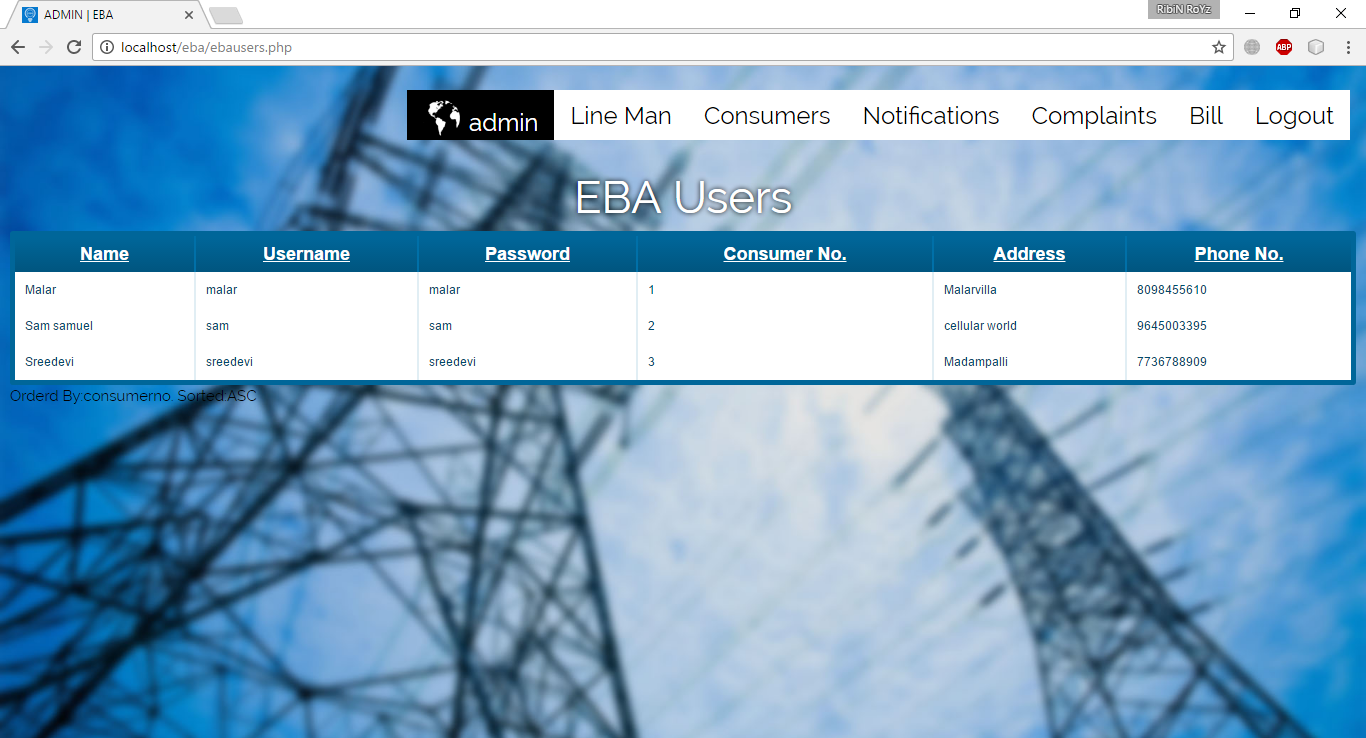
\includegraphics[width=10cm ,height=5.9cm]{ebausers.png} 
%\caption{ER Diagram}
\end{figure}
\end{frame}

\begin{frame}
\frametitle{Consumers }
\begin{figure}[center]
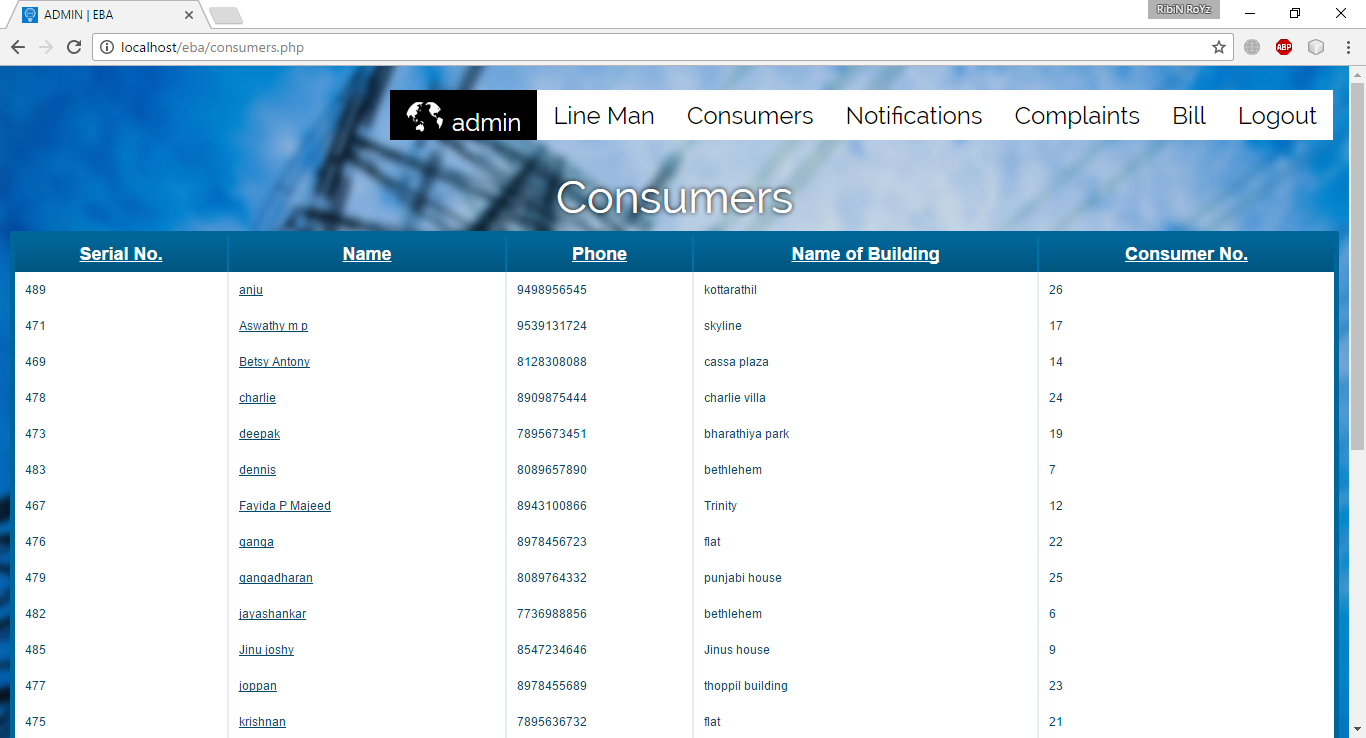
\includegraphics[width=10cm ,height=5.9cm]{consumers.png} 
%\caption{ER Diagram}
\end{figure}
\end{frame}

\begin{frame}
\frametitle{Consumer Details}
\begin{figure}[center]
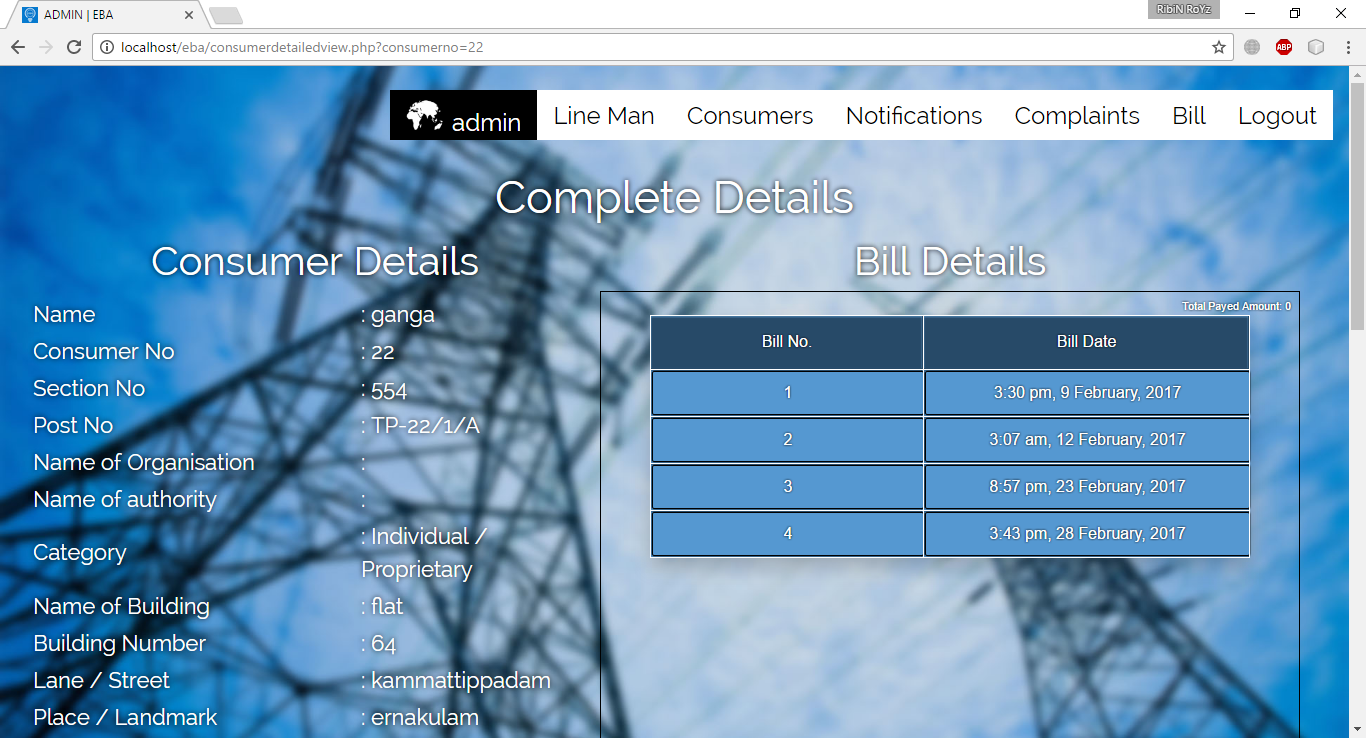
\includegraphics[width=10cm ,height=5.9cm]{consumerdetails.png} 
%\caption{ER Diagram}
\end{figure}
\end{frame}

\begin{frame}
\frametitle{Add Notification}
\begin{figure}[center]
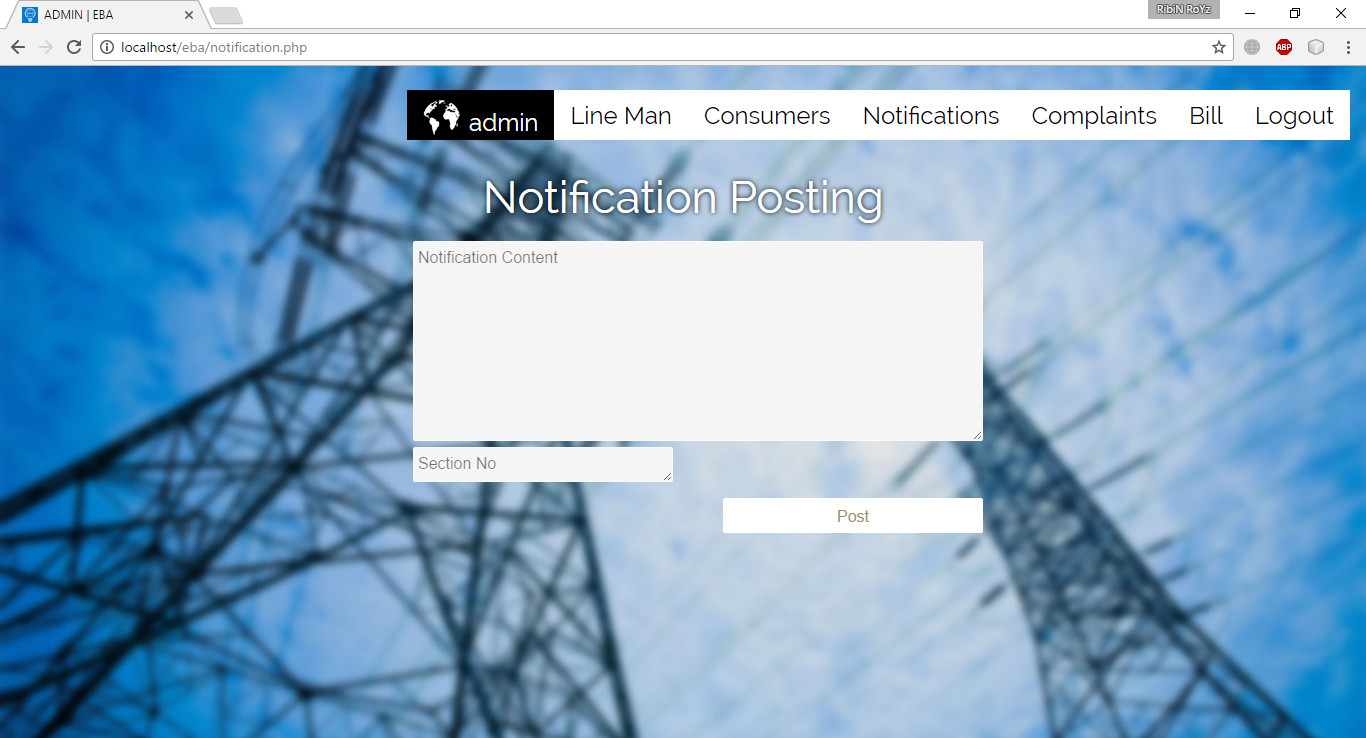
\includegraphics[width=10cm ,height=5.9cm]{notificationadd.png} 
%\caption{ER Diagram}
\end{figure}
\end{frame}

\begin{frame}
\frametitle{Notification View}
\begin{figure}[center]
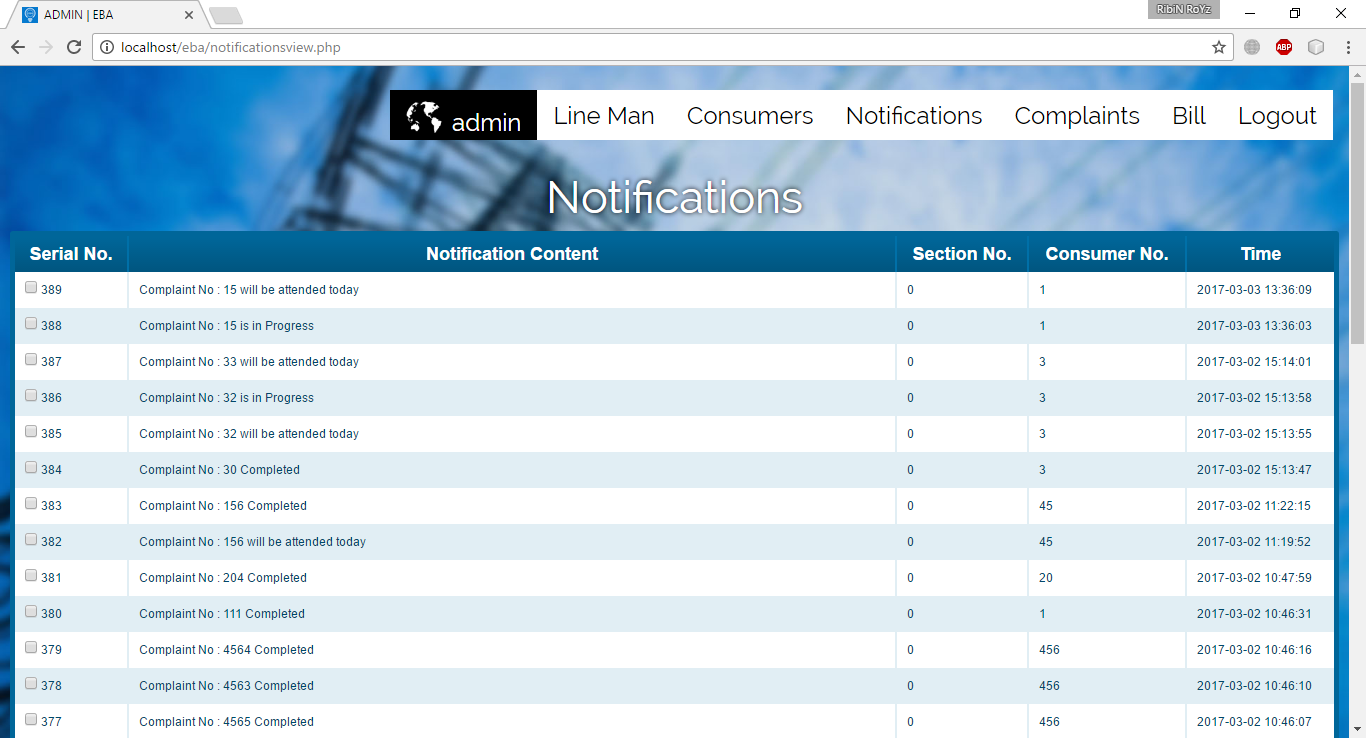
\includegraphics[width=10cm ,height=5.9cm]{notificationview.png} 
%\caption{ER Diagram}
\end{figure}
\end{frame}

\begin{frame}
\frametitle{Complaint New}
\begin{figure}[center]
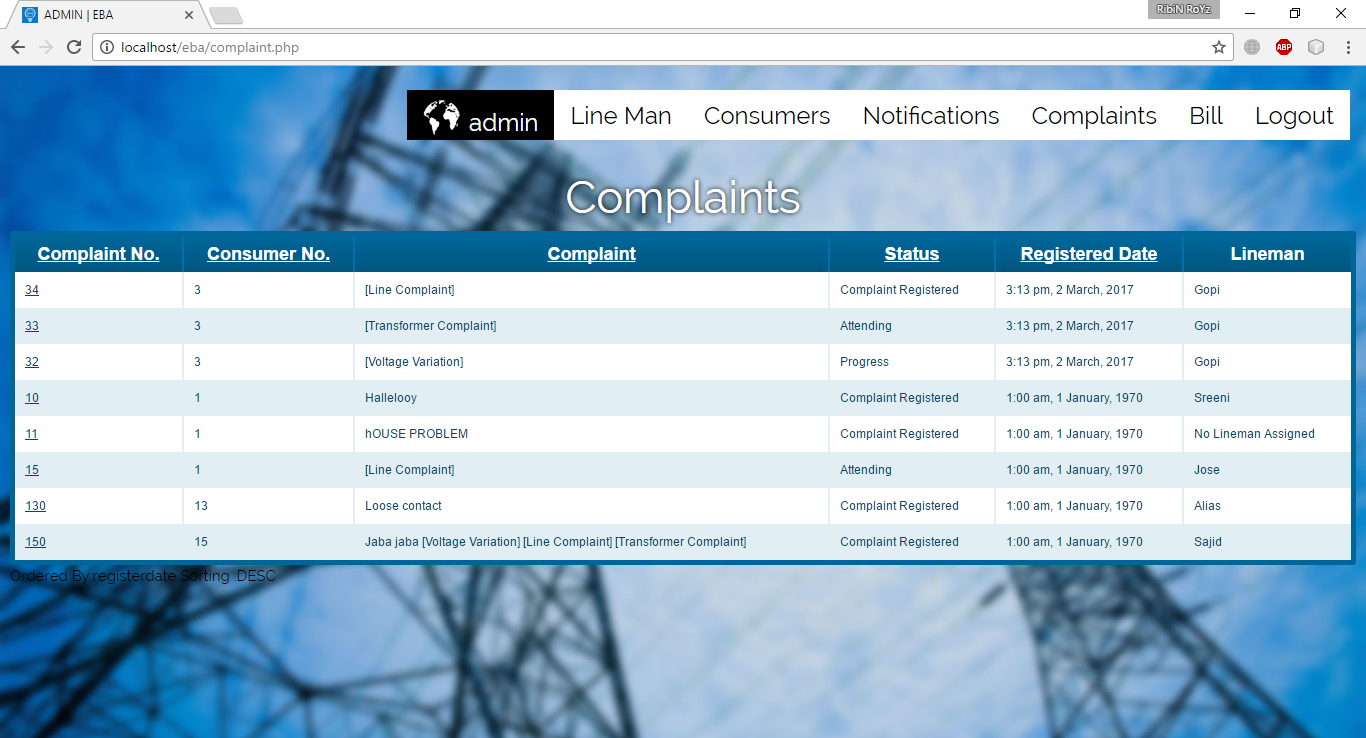
\includegraphics[width=10cm ,height=5.9cm]{complaintnew.png} 
%\caption{ER Diagram}
\end{figure}
\end{frame}

\begin{frame}
\frametitle{Complaint Single}
\begin{figure}[center]
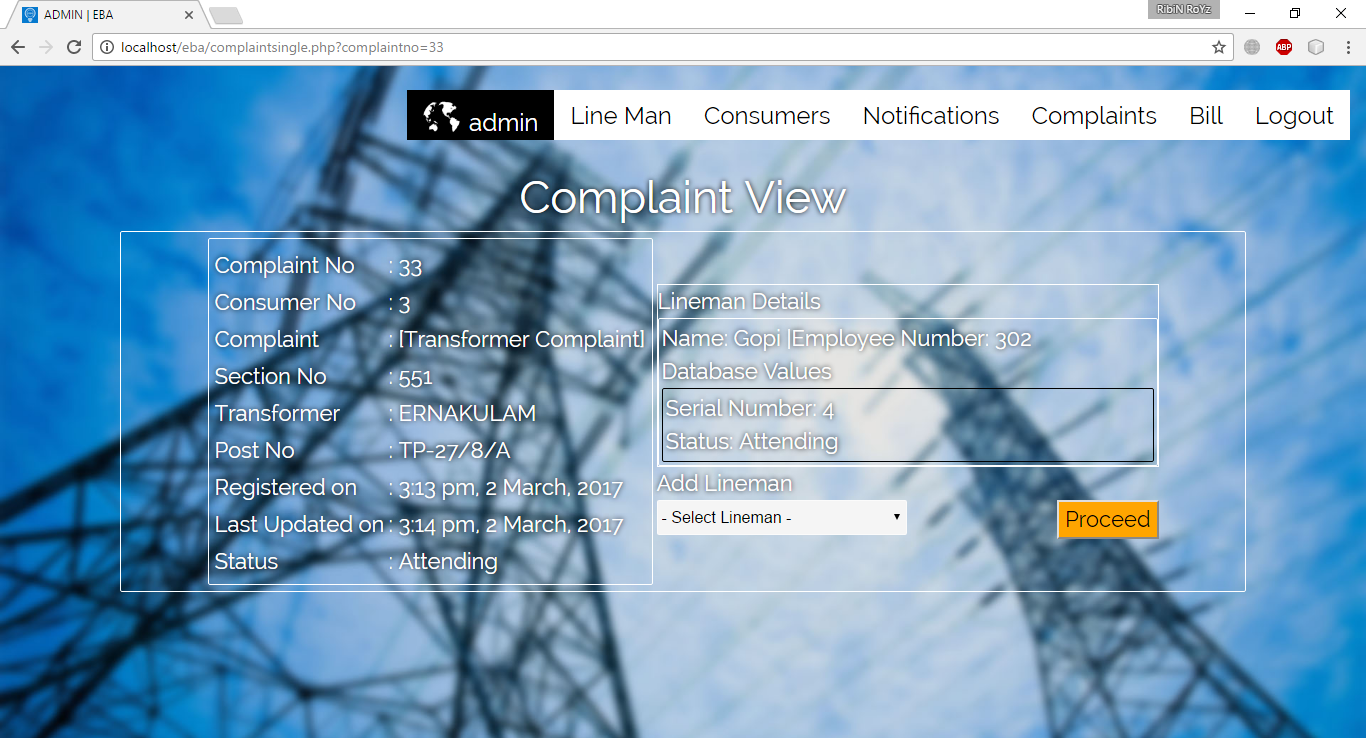
\includegraphics[width=10cm ,height=5.9cm]{complaintsingle.png} 
%\caption{ER Diagram}
\end{figure}
\end{frame}

\begin{frame}
\frametitle{Complaint History}
\begin{figure}[center]
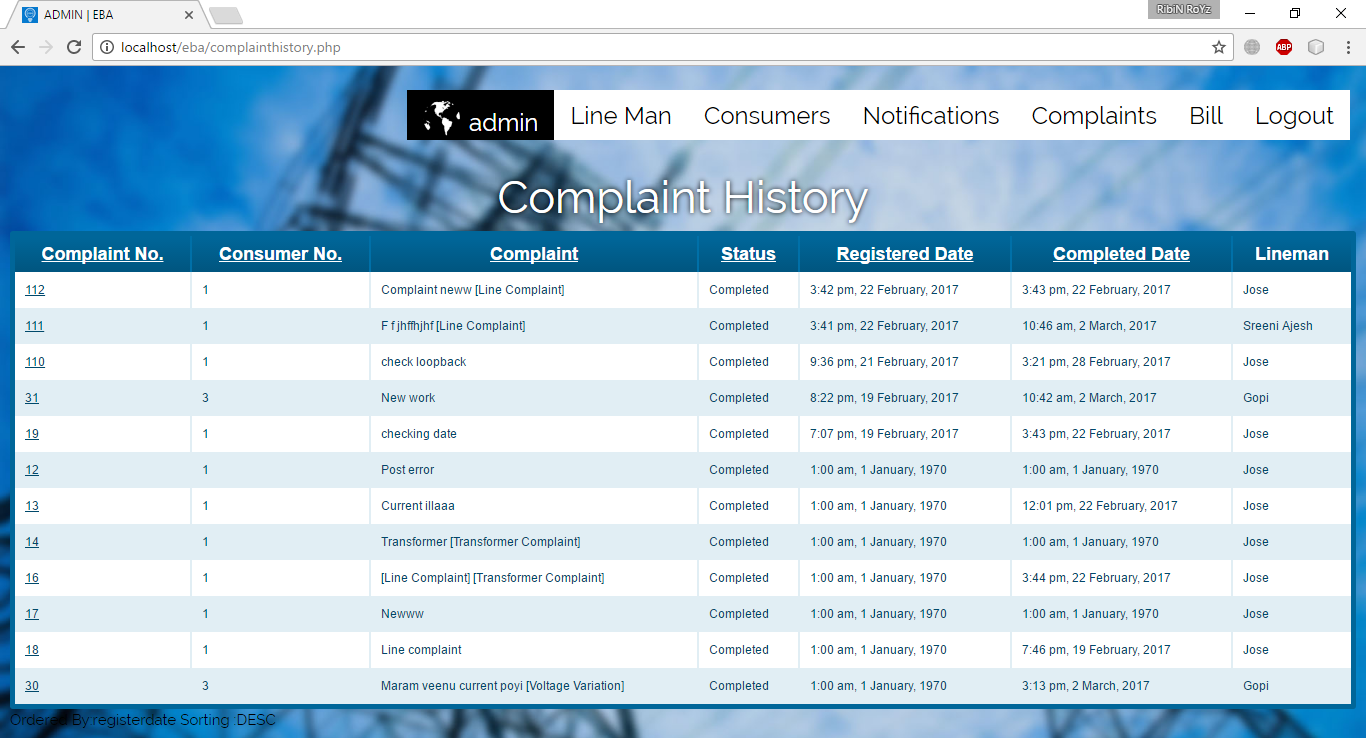
\includegraphics[width=10cm ,height=5.9cm]{complainthistory.png} 
%\caption{ER Diagram}
\end{figure}
\end{frame}

\begin{frame}
\frametitle{Bill Update}
\begin{figure}[center]
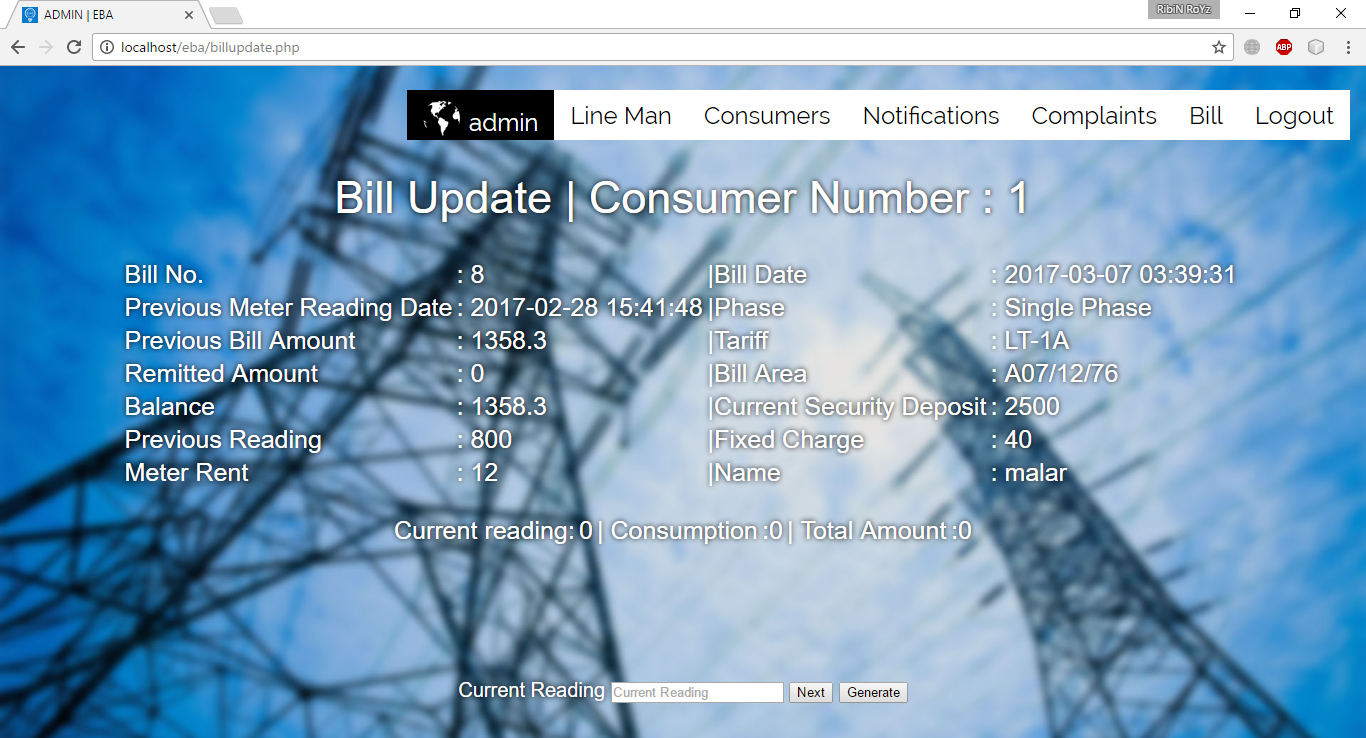
\includegraphics[width=10cm ,height=5.9cm]{billupdate.png} 
%\caption{ER Diagram}
\end{figure}
\end{frame}

\begin{frame}
\frametitle{Bill Due}
\begin{figure}[center]
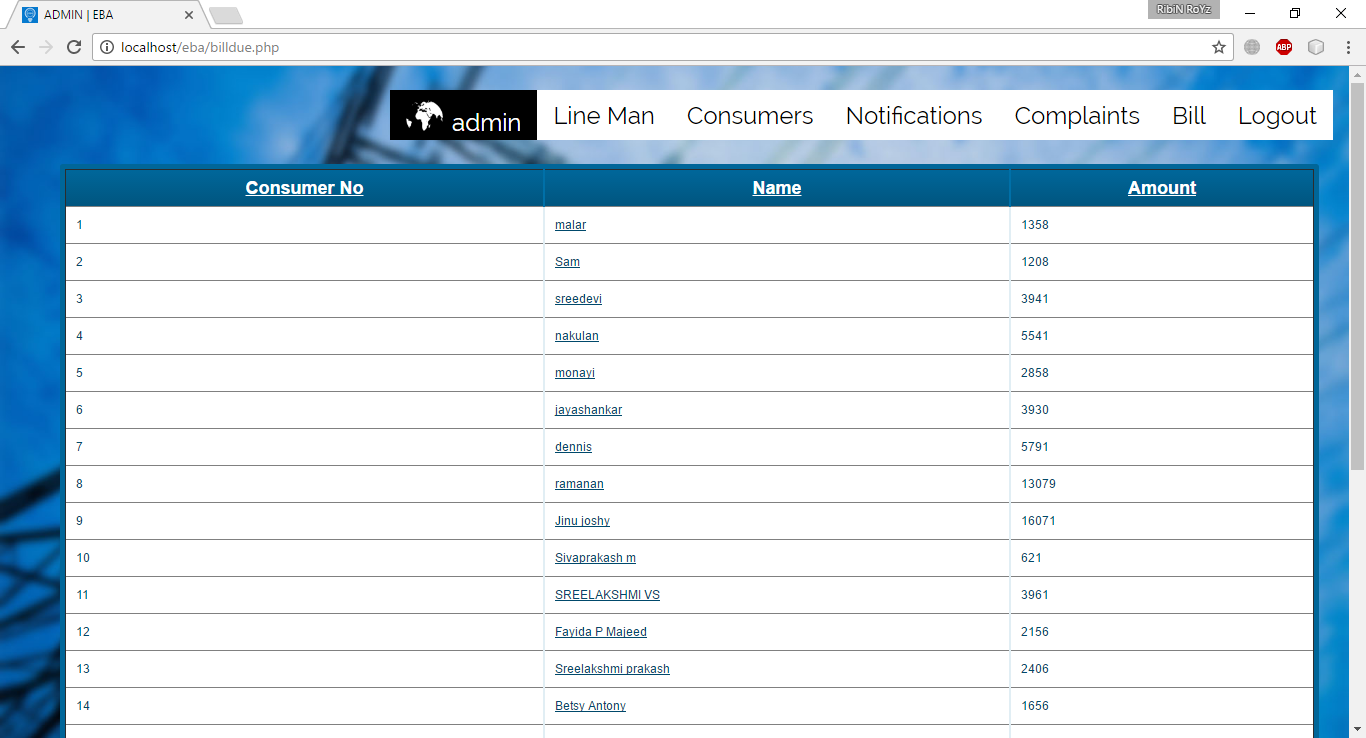
\includegraphics[width=10cm ,height=5.9cm]{billdue.png} 
%\caption{ER Diagram}
\end{figure}
\end{frame}

\begin{frame}
\frametitle{IMPLEMENTATION}
\begin{itemize}
\item The languages used are:
\begin{itemize}
	\item PHP: PHP is a server-side scripting language designed primarily for web development but is also used as a general-purpose programming language.
	\item JAVA: Java is a general-purpose computer programming language that is concurrent, class based, object-oriented, and specifically designed to have as few implementation dependencies as possible.
	\item Android: Android is a mobile operating system developed by Google, based on the Linux kernel and designed primarily for touch screen mobile devices such as smart phones and tablets
\end{itemize}
\end{itemize}
\end{frame}
\begin{frame}
\frametitle {CONCLUSION }
\begin{itemize}
	\item Proposed system is more user friendly.
	\item User will get informations about his/her current connection.
	\item User can pay bill easily.
	\item User can easily report their issues related to current connection.
	
	
\end{itemize}
\end{frame}


\begin{frame}
\frametitle {CONCLUSION Cont.. }
\begin{itemize}
	\item Lineman get the complaint at the same time a complaint is booked.
	\item Live Complaint Status facility
	\item Same application to support both lineman/consumers
	\item Moreover, all the services associated with the electricity board is collaborated into a single device.
		
	
\end{itemize}
\end{frame}

\begin{frame}
\frametitle {REFERENCES}
\begin{itemize}

 \item Stack Overflow. \textit{http://www.Stackoverflow.com/}
 \item Tutorial Point. \textit{http://www.tutorialspoint.com/}
  \item w3schools.
  \textit{http://www.w3schools.com/}
   \item Android developers.
    \textit{http:/developer.android.com/}
    \item Youtube.
        \textit{http:/www.youtube.com/}
    \item tizag.com.
        \textit{http:/www.tizaq.com/}
        \item IO Draw. \textit{http://www.draw.io.com/}
        \item Github. \textit{http://www.github.com/}
        \item Codeguru. \textit{http://www.codeguru.com/}
        \item Nestpia. \textit{http://www.nestpia.com/}

	
\end{itemize}
\end{frame}



\begin{frame}
\begin{center}
\begin{figure}[center]

\includegraphics[width=8cm,height=6.5cm]{tu.jpg}
\end{figure}
\end{center}
\end{frame}



\end{document}

